% TEMPLATE for Usenix papers, specifically to meet requirements of
%  USENIX '05
% originally a template for producing IEEE-format articles using LaTeX.
%   written by Matthew Ward, CS Department, Worcester Polytechnic Institute.
% adapted by David Beazley for his excellent SWIG paper in Proceedings,
%   Tcl 96
% turned into a smartass generic template by De Clarke, with thanks to
%   both the above pioneers
% use at your own risk.  Complaints to /dev/null.
% make it two column with no page numbering, default is 10 point

% Munged by Fred Douglis <douglis@research.att.com> 10/97 to separate
% the .sty file from the LaTeX source template, so that people can
% more easily include the .sty file into an existing document.  Also
% changed to more closely follow the style guidelines as represented
% by the Word sample file. 
% This version uses the latex2e styles, not the very ancient 2.09 stuff.
\documentclass[letterpaper,twocolumn,10pt]{article}
\usepackage{usenix,epsfig,endnotes,xspace,color}

% Name candidates:
%  Anza
%  Void 
%  Station (from Genesis's Grand Central component) 
%  TARDIS: Atomic, Recoverable, Datamodel Independent Storage
% EAB: flex, basis, stable, dura
% Stasys:  SYStem for Adaptable Transactional Storage: 

\newcommand{\yad}{Stasis\xspace}
\newcommand{\yads}{Stasis'\xspace}
\newcommand{\oasys}{Oasys\xspace}

\newcommand{\diff}[1]{\textcolor{blue}{\bf #1}}
\newcommand{\eab}[1]{\textcolor{red}{\bf EAB: #1}}
\newcommand{\rcs}[1]{\textcolor{green}{\bf RCS: #1}}
%\newcommand{\mjd}[1]{\textcolor{blue}{\bf MJD: #1}}

\newcommand{\eat}[1]{}

\begin{document}

%don't want date printed
\date{}


%make title bold and 14 pt font (Latex default is non-bold, 16 pt)
\title{\Large \bf \yad: System for Adaptable, Transactional Storage}

%for single author (just remove % characters)
\author{
{\rm Russell Sears}\\
UC Berkeley
\and
{\rm Eric Brewer}\\
UC Berkeley
} % end author

\maketitle

% Use the following at camera-ready time to suppress page numbers.
% Comment it out when you first submit the paper for review.
%\thispagestyle{empty}


%\subsection*{Abstract}

{\em An increasing range of applications requires robust support for atomic, durable and concurrent
transactions.  Databases provide the default solution, but force
applications to interact via SQL and to forfeit control over data
layout and access mechanisms.  We argue there is a gap between DBMSs and file systems that limits designers of data-oriented applications.

\yad is a storage framework that incorporates ideas from traditional
write-ahead-logging storage algorithms and file systems.
It provides applications with flexible control over data structures, data layout, performance and robustness properties.
\yad enables the development of
unforeseen variants on transactional storage by generalizing
write-ahead-logging algorithms.  Our partial implementation of these
ideas already provides specialized (and cleaner) semantics to applications.

We evaluate the performance of a traditional transactional storage
system based on \yad, and show that it performs favorably relative to existing
systems.  We present examples that make use of custom access methods, modified
buffer manager semantics, direct log file manipulation, and LSN-free
pages.  These examples facilitate sophisticated performance 
optimizations such as zero-copy I/O.  These extensions are composable,
easy to implement and significantly improve performance.

}
%We argue that our ability to support such a diverse range of
%transactional systems stems directly from our rejection of
%assumptions made by early database designers.  These assumptions
%permeate ``database toolkit'' research.  We attribute the success of
%low-level transaction processing libraries (such as Berkeley DB) to
%a partial break from traditional database dogma.

% entries, and 
% to reduce memory and
%CPU overhead, reorder log entries for increased efficiency, and do
%away with per-page LSNs in order to perform zero-copy transactional
%I/O.  
%We argue that encapsulation allows applications to compose
%extensions.

%These ideas have been partially implemented, and initial performance
%figures, and experience using the library compare favorably with
%existing systems.



\section{Introduction}

As our reliance on computing infrastructure increases, a wider range
of applications requires robust data management.  Traditionally, data
management has been the province of database management systems
(DBMSs), which are well-suited to enterprise applications, but lead to
poor support for systems such as web services, search engines, version
systems, work-flow applications, bioinformatics, and
scientific computing.  These applications have complex transactional
storage requirements, but do not fit well onto SQL or the monolithic
approach of current databases.  In fact, when performance matters
these applications often avoid DBMSs and instead implement ad-hoc data
management solutions on top of file systems.

An example of this mismatch is in the support for persistent objects.
In a typical usage, an array of objects is made persistent by mapping
each object to a row in a table (or sometimes multiple
tables)~\cite{hibernate} and then issuing queries to keep the objects
and rows consistent. An update must confirm it has the current
version, modify the object, write out a serialized version using the
SQL update command, and commit.  Also, for efficiency, most systems
must buffer two copies of the application's working set in memory.
This is an awkward and inefficient mechanism, and hence we claim that
DBMSs do not support this task well.

Bioinformatics systems perform complex scientific computations over
large, semi-structured databases with rapidly evolving schemas.
Versioning and lineage tracking are also key concerns.  Relational
databases support none of these requirements well.  Instead, office
suites, ad-hoc text-based formats and Perl scripts are used for data
management~\cite{perl}, with mixed success~\cite{excel}.

Our hypothesis is that 1) each of these areas has a distinct top-down
conceptual model (which may not map well to the relational model); and
2) there exists a bottom-up layered framework that can better support all of these
models and others. 

Just within databases, relational, object-oriented, XML, and streaming
databases all have distinct conceptual models.  Scientific computing,
bioinformatics and version-control systems tend to avoid
update-in-place and track provenance and thus have a distinct
conceptual model.  Search engines and data warehouses in theory can
use the relational model, but in practice need a very different
implementation.


%Simply providing
%access to a database system's internal storage module is an improvement.
%However, many of these applications require special transactional properties 
%that general-purpose transactional storage systems do not provide.  In
%fact, DBMSs are often not used for these systems, which instead
%implement custom, ad-hoc data management tools on top of file
%systems.

\eat{
Examples of real world systems that currently fall into this category
are web search engines, document repositories, large-scale web-email
services, map and trip planning services, ticket reservation systems,
photo and video repositories, bioinformatics, version control systems,
work-flow applications, CAD/VLSI applications and directory services.

In short, we believe that a fundamental architectural shift in
transactional storage is necessary before general-purpose storage
systems are of practical use to modern applications.
Until this change occurs, databases' imposition of unwanted
abstraction upon their users will restrict system designs and
implementations.
}

To explore this hypothesis, we present \yad, a library that provides transactional
storage at a level of abstraction as close to the hardware as
possible.  The library can support special-purpose, transactional
storage models in addition to ACID database-style interfaces to
abstract data models.  \yad incorporates techniques from databases
(e.g. write-ahead logging) and operating systems (e.g. zero-copy techniques).

Our goal is to combine the flexibility and layering of low-level
abstractions typical for systems work with the complete semantics
that exemplify the database field.
By {\em flexible} we mean that \yad{}  can support a wide
range of transactional data structures {\em efficiently}, and that it can support a variety
of policies for locking, commit, clusters and buffer management.
Also, it is extensible for new core operations
and new data structures. It is this flexibility that allows the
support of a wide range of systems and models.

By {\em complete} we mean full redo/undo logging that supports
both {\em no force}, which provides durability with only log writes,
and {\em steal}, which allows dirty pages to be written out prematurely
to reduce memory pressure. By complete, we also
mean support for media recovery, which is the ability to roll
forward from an archived copy, and support for error-handling,
clusters, and multithreading. These requirements are difficult
to meet and form the {\em raison d'\^etre} for \yad{}: the framework
delivers these properties as reusable building blocks for systems
that implement complete transactions.

Through examples and their good performance, we show how \yad{}
efficiently supports a wide range of uses that fall in the gap between 
database and file system technologies, including
persistent objects, graph- or XML-based applications, and recoverable
virtual memory~\cite{lrvm}.  

For example, on an object serialization workload, we provide up to 
a 4x speedup over an in-process MySQL implementation and a 3x speedup over Berkeley DB, while 
cutting memory usage in half (Section~\ref{sec:oasys}). 
We implemented this extension in 150 lines of C, including comments and boilerplate.  We did not have this type of optimization
in mind when we wrote \yad, and in fact the idea came from a
user unfamiliar with \yad.

%\e ab{others?  CVS, windows registry, berk DB, Grid FS?}
%\r cs{maybe in related work?}

This paper begins by contrasting \yads approach with that of
conventional database and transactional storage systems.  It proceeds
to discuss write-ahead logging, and describe ways in which \yad can be
customized to implement many existing (and some new) write-ahead
logging variants.  We present implementations of some of these variants and
benchmark them against popular real-world systems.  We
conclude with a survey of the technologies upon which \yad is based.

An (early) open-source implementation of
the ideas presented here is available at \eab{where?}.

\section{\yad is not a Database}
\label{sec:notDB}

Database research has a long history, including the development of
many technologies that our system builds upon.  This section explains
why databases are fundamentally inappropriate tools for system
developers, and covers some of the preivous responses of the systems
community.  The problems we present here have been the focus of
database and systems researchers for at least 25 years.

\subsection{The Database View}

The database community approaches the limited range of DBMSs by either
creating new top-down models, such as XML databases or streaming
databases, or by extending the relational model~\cite{codd} along some axis, such
as new data types.  (We cover these attempts in more detail in
Section~\ref{related-work}.) \eab{add cites}

%Database systems are often thought of in terms of the high-level
%abstractions they present.  For instance, relational database systems
%implement the relational model~\cite{codd}, object-oriented
%databases implement object abstractions \eab{[?]}, XML databases implement
%hierarchical datasets~\eab{[?]}, and so on.  Before the relational model,
%navigational databases implemented pointer- and record-based data models.

An early survey of database implementations sought to enumerate the
fundamental components used by database system implementors~\cite{batoryConceptual,batoryPhysical}.  This
survey was performed due to difficulties in extending database systems
into new application domains.  It divided internal database
routines into two broad modules: {\em conceptual mappings} and {\em physical
database models}.

%A physical model would then translate a set of tuples into an
%on-disk B-Tree, and provide support for iterators and range-based query
%operations.

It is the responsibility of a database implementor to choose a set of
conceptual mappings that implement the desired higher-level
abstraction (such as the relational model).  The physical data model
is chosen to support efficiently the set of mappings that are built on
top of it.

A conceptual mapping based on the relational model might translate a
relation into a set of keyed tuples.  If the database were going to be
used for short, write-intensive and high-concurrency transactions
(OLTP), the physical model would probably translate sets of tuples
into an on-disk B-Tree.  In contrast, if the database needed to
support long-running, read-only aggregation queries (OLAP) over high
dimensional data, a physical model that stores the data in a sparse
array format would be more appropriate~\cite{molap}.  Although both
OLTP and OLAP databases are based upon the relational model they make
use of different physical models in order to serve different classes
of applications.

A basic claim of
this paper is that no single known physical data model can efficiently
support the wide range of conceptual mappings that are in use today.
In addition to sets, objects, and XML, such a model would need
to cover search engines, version-control systems, work-flow
applications, and scientific computing, as examples.

Instead of attempting to create such a unified model after decades of
database research has failed to produce one, we opt to provide a
bottom-up transactional toolbox that supports many different models
efficiently.  This makes it easy for system designers to
implement most of the data models that the underlying hardware can
support, or to abandon the database approach entirely, and forgo the
use of a structured physical model and abstract conceptual mappings.

\subsection{The Systems View}

The systems community has also worked on this mismatch for 20 years,
which has led to many interesting projects.  Examples include
alternative durability models such as Quicksilver or LRVM, persistent
objects systems such as Argus, and cluster hash tables [add cites].
We expect that \yad would simplify the implementation of most if not
all of these systems.  We look at these in more detail in
Section~\ref{related=work}.

In some sense, our hypothesis is trivially true in that there exists a
bottom-up framework called the ``operating system'' that can implement
all of the models. A famous database paper argues that it does so
poorly (Stonebraker 1980~\cite{Stonebraker80}). Our task is really to
simplify the implementation of transactional systems through more
powerful primitives that enable concurrent transactions with a variety
of performance/robustness tradeoffs.

The closest system to ours in spirit is Berkley DB,  a highly successful alternative to conventional
databases~\cite{libtp}.  At its core, it provides the physical database model
(relational storage system~\cite{systemR}) of a conventional database server.
%It is based on the
%observation that the storage subsystem is a more general (and less
%abstract) component than a monolithic database, and provides a
%stand-alone implementation of the storage primitives built into 
%most relational database systems~\cite{libtp}.  
In particular, 
it provides fully transactional (ACID) operations over B-Trees, 
hash tables, and other access methods.  It provides flags that 
let its users tweak various aspects of the performance of these
primitives, and selectively disable the features it provides.

With the exception of the benchmark designed to fairly compare the two
systems, none of the \yad applications presented in
Section~\ref{sec:extensions} are efficiently supported by Berkeley DB.
This is a result of Berkeley DB's assumptions regarding workloads and
decisions regarding low-level data representation.  Thus, although
Berkeley DB could be built on top of \yad, Berkeley DB's data model
and write-ahead logging system are too specialized to support \yad.




\section{Conventional Transactions in \yad}

\rcs{This section is missing references to prior work.  Bill mentioned
PhD theses that talk about this layering, but I've been too busy
coding to read them.}

This section describes how \yad implements transactions that are
similar to those provided by relational database systems.  In addition
to providing a review of how modern transactional systems function,
this section lays out the functionality that \yad provides to the
operations built on top of it.  It also explains how \yads
operations are roughly structured as two levels of abstraction.  

The transcational algorithms described in this section are not at all
novel, and are in fact based on ARIES~\cite{aries}.  However, they
provide important background.  There is a large body of literature
explaining optimizations and implementation techniques related to this
type of recovery algorithm.  Any good database textbook would cover these
issues in more detail.

The lower level of a \yad operation provides atomic
updates to regions of the disk.  These updates do not have to deal
with concurrency, but the portion of the page file that they read and
write must be updated atomically, even if the system crashes.

The higher-level provides operations that span multiple pages by
atomically applying sets of operations to the page file and coping
with concurrency issues.  Surprisingly, the implementations of these
two layers are only loosely coupled.

Finally, this section describes how \yad manages transaction-duration
locks and discusses the alternatives \yad provides to application developers.

\subsection{Atomic page file operations}

Transactional storage algorithms work because they are able to
update atomically portions of durable storage.  These small atomic
updates are used to bootstrap transactions that are too large to be
applied atomically.  In particular, write-ahead logging (and therefore
\yad) relies on the ability to atomically write entries to the log
file.

\subsubsection{Hard drive behavior during a crash}
In practice, a write to a disk page is not atomic.  Two common failure
modes exist.  The first occurs when the disk writes a partial sector
during a crash.  In this case, the drive maintains an internal
checksum, detects a mismatch, and reports it when the page is read.
The second case occurs because pages span multiple sectors.  Drives
may reorder writes on sector boundaries, causing an arbitrary subset
of a page's sectors to be updated during a crash.  {\em Torn page
detection} can be used to detect this phenomonon.

Torn
and corrupted pages may be recovered by using {\em media recovery} to
restore the page from backup.  Media recovery works by reinitializing
the page to zero, and playing back the REDO entries in the log that
modify the page.  In practice, a system administrator would
periodically back up the page file, thus enabling log truncation and
shortening recovery time.

For simplicity, this section ignores mechanisms that detect
and restore torn pages, and assumes that page writes are atomic.
Although the techniques described in this section rely on the ability to
update disk pages atomically, this restriction is relaxed by other 
recovery mechanisms.


\subsubsection{Extending \yad with new operations}

Figure~\ref{fig:structure} shows how operations interact with \yad.  A
number of default operations come with \yad.  These include operations
that allocate and manipulate records, operations that implement hash
tables, and a number of methods that add functionality to recovery.

If an operation does not need to be used by concurrent
transactions, directly manipulating the page file is as simple as
ensuring that each update to the page file occurs inside of the
operation's implementation.  Operation implementations must be invoked
by registering a callback with \yad at startup, and then calling {\em
Tupdate()} to invoke the operation at runtime.  

Each operation should be deterministic, provide an inverse, and
acquire all of its arguments from a struct that is passed via
Tupdate() and from the page it updates.  The callbacks that are used
during forward opertion are also used during recovery.  Therefore
operations provide a single redo function and a single undo function.
(There is no ``do'' function.)  This reduces the amount of
recovery-specific code in the system.  Tupdate() writes the struct
that is passed to it to the log before invoking the operation's
implementation.  Recovery simply reads the struct from disk and passes
it into the operation implementation.

In this portion of the discussion, operations are limited
to a single page, and provide an undo function.  Operations that
affect multiple pages or do not provide inverses will be
discussed later.

Operations are limited to a single page because their results must be
applied to the page file atomically.  Some operations use the data
stored on the page to update the page.  If this data were corrupted by
a non-atomic disk write, then such operations would fail during recovery.

Note that we could implement a limited form of transactions by
limiting each transaction to a single operation, and by forcing the
page that each operation updates to disk in order.  If we ignore torn 
pages and failed sectors, this does not
require any sort of logging, but is quite inefficient in practice, as
it forces the disk to perform a potentially random write each time the
page file is updated.  The rest of this section describes how recovery
can be extended, first to support multiple operations per
transaction efficiently, and then to allow more than one transaction to modify the
same data before committing.

\subsubsection{\yads Recovery Algorithm}

Recovery relies upon the fact that each log entry is assigned a {\em
Log Sequence Number (LSN)}.  The LSN is monitonically increasing and
unique.  The LSN of the log entry that was most recently applied to
each page is stored with the page, which allows recovery to replay log entries selectively.  This only works if log entries change exactly one
page and if they are applied to the page atomically.

Recovery occurs in three phases, Analysis, Redo and Undo.
``Analysis'' is beyond the scope of this paper, but essentially determines the commit/abort status of every transaction.  ``Redo'' plays the
log forward in time, applying any updates that did not make it to disk
before the system crashed.  ``Undo'' runs the log backwards in time,
only applying portions that correspond to aborted transactions.  This
section only considers physical undo.  Section~\ref{sec:nta} describes
the distinction between physical and logical undo.
A summary of the stages of recovery and the invariants
they establish is presented in Figure~\ref{fig:conventional-recovery}.

Redo is the only phase that makes use of LSNs stored on pages.
It simply compares the page LSN to the LSN of each log entry.  If the
log entry's LSN is higher than the page LSN, then the log entry is
applied.  Otherwise, the log entry is skipped.  Redo does not write
log entries to disk, as it is replaying events that have already been
recorded.  

However, Undo does write log entries.  In order to prevent repeated
crashes during recovery from causing the log to grow excessively, the
entries that Undo writes tell future invocations of Undo to skip
portions of the transaction that have already been undone.  These log
entries are usually called {\em Compensation Log Records (CLRs)}.
Note that CLRs only cause Undo to skip log entries.  Redo will apply
log entries protected by the CLR, guaranteeing that those updates are
applied to the page file.

There are many other schemes for page-level recovery that we could
have chosen.  The scheme desribed above has two particularly nice
properties.  First, pages that were modified by active transactions
may be {\em stolen}; they may be written to disk before a transaction
completes.  This allows transactions to use more memory than is
physically available, and makes it easier to flush frequently written
pages to disk.  Second, pages do not need to be {\em forced}; a
transaction commits simply by flushing the log.  If it had to force
pages to disk it would incur the cost of random I/O.  Also, if
multiple transactions commit in a small window of time, the log only
needs to be forced to disk once.

\subsubsection{Alternatives to Steal / no-Force}

Note that the Redo phase of recovery allows \yad to avoid forcing
pages to disk, while Undo allows pages to be stolen.  For some
applications, the overhead of logging information for Redo or Undo may
outweigh their benefits.  \yads logging discipline provides a simple
solution to this problem.  If a special-purpose operation wants to
avoid writing either the Redo or the Undo information to the log then
it can have the buffer manager pin the page or flush it at commit, and
simply omit the pertinent information from the log entries it
generates.

Recovery's Undo and Redo phases both will process the log entry, but
one of them will have no effect.  If an operation chooses not to
provide a Redo implementation, then its Undo implementation will need
to determine whether or not the Redo was applied.  If it omits Undo,
then Redo must consult recovery to see if it is part of a transaction that
committed.

\subsection{Concurrent Transactions}

Two factors make it more difficult to write operations that may be
used in concurrent transactions.  The first is familiar to anyone that
has written multi-threaded code: Accesses to shared data structures
must be protected by latches (mutexes).  The second problem stems from
the fact that concurrent transactions prevent abort from simply
rolling back the physical updates that a transaction made.
Fortunately, it is straightforward to reduce this second,
transaction-specific, problem to the familiar problem of writing
multi-threaded software.  \diff{In this paper, ``concurrent transactions''
are transactions that perform interleaved operations.  They do not
necessarily exploit the parallelism provided by multiprocessor
systems.}

To understand the problems that arise with concurrent transactions,
consider what would happen if one transaction, A, rearranged the
layout of a data structure.  Next, assume a second transaction, B,
modified that structure, and then A aborted.  When A rolls back, its
UNDO entries will undo the rearrangement that it made to the data
structure, without regard to B's modifications.  This is likely to
cause corruption.

Two common solutions to this problem are {\em total isolation} and
{\em nested top actions}.  Total isolation simply prevents any
transaction from accessing a data structure that has been modified by
another in-progress transaction.  An application can achieve this
using its own concurrency control mechanisms, or by holding a lock on
each data structure until the end of the transaction.  Releasing the
lock after the modification, but before the end of the transaction,
increases concurrency.  However, it means that follow-on transactions that use
that data may need to abort if a current transaction aborts ({\em
cascading aborts}).  %Related issues are studied in great detail in terms of optimistic concurrency control~\cite{optimisticConcurrencyControl, optimisticConcurrencyPerformance}.

Unfortunately, the long locks held by total isolation cause
bottlenecks when applied to key data structures.  Nested top actions
are essentially mini-transactions that can commit even if their
containing transaction aborts; thus follow-on transactions can use the
data structure without fear of cascading aborts.

The key idea is to distinguish between the {\em logical operations} of a
data structure, such as inserting a key, and the {\em physical operations}
such as splitting tree nodes or rebalancing a tree. The physical
operations do not need to be undone if the containing logical operation
(e.g. {\em insert}) aborts.  \diff{We record such operations using {\em logical 
logging} and {\em physical logging}, respectively.}

\diff{Each nested top action performs a single logical operation by
applying a number of physical operations to the page file.  Physical
REDO and UNDO log entries are stored in the log so that recovery can
repair any temporary inconsistency that the nested top action
introduces.  Once the nested top action has completed, a logical UNDO
entry is recorded, and a CLR is used to tell recovery to ignore the
physical UNDO entries.  This logical UNDO can then be safely applied
even after other transactions manipulate the data structure.  If the
nested transaction does not complete, physical UNDO can safely roll
back the changes.  Therefore, nested transactions can always be rolled
back as long as the physical updates are protected from other
transactions and complete nested transactions preserve the integrity
of the structures they manipulate.}

This leads to a mechanical approach that converts non-reentrant
operations that do not support concurrent transactions into reentrant,
concurrent operations:

\begin{enumerate}
\item Wrap a mutex around each operation.  With care, it is possible 
  to use finer-grained latches in a \yad operation, but it is rarely necessary.
\item Define a {\em logical} UNDO for each operation (rather than just
  using a set of page-level UNDO's).  For example, this is easy for a
  hash table: the UNDO for {\em insert} is {\em remove}.  This logical
  undo function should arrange to acquire the mutex when invoked by
  abort or recovery.
\item Add a ``begin nested top action'' right after the mutex
  acquisition, and an ``end nested top action'' right before the mutex
  is released.  \yad includes operations that provide nested top
  actions.
\end{enumerate}

If the transaction that encloses a nested top action aborts, the
logical undo will {\em compensate} for the effects of the operation,
leaving structural changes intact.  If a transaction should perform
some action regardless of whether or not it commits, a nested top
action with a ``no-op'' as its inverse is a convenient way of applying
the change.  Nested top actions do not cause the log to be forced to disk, so
such changes will not be durable until the log is manually forced, or
until the updates eventually reach disk.

This section described how concurrent, thread-safe operations can be
developed.  These operations provide building blocks for concurrent
transactions, and are fairly easy to develop.  Therefore, they are
used throughout \yads default data structure implementations.  

Interestingly, any mechanism that applies atomic physical updates to
the page file can be used as the basis of a nested top action.
However, concurrent operations are of little help if an application is
not able to safely combine them to create concurrent transactions.

\subsection{Application-specific Locking}

Note that the transactions described above only provide the
``Atomicity'' and ``Durability'' properties of ACID.\endnote{The ``A'' in ACID really means atomic persistence
of data, rather than atomic in-memory updates, as the term is normally
used in systems work~\cite{GR97}; 
the latter is covered by ``C'' and
``I''.}  ``Isolation'' is
typically provided by locking, which is a higher-level but
comaptible layer.  ``Consistency'' is less well defined but comes in
part from low-level mutexes that avoid races, and partially from
higher-level constructs such as unique key requirements.  \yad
supports this by distinguishing between {\em latches} and {\em locks}.
Latches are provided using operating system mutexes, and are held for
short periods of time.  \yads default data structures use latches in a
way that avoids deadlock.  This section will describe \yads latching
protocols and describes two custom lock
managers that \yads allocation routines use to implement layout 
policies and provide deadlock avoidance.  Applications that want
conventional transactional isolation (serializability) can make 
use of a lock manager.  Alternatively, applications may follow 
the example of \yads default data structures, and implement 
deadlock avoidance, or other custom lock management schemes.\rcs{Citations here?}

This allows higher-level code to treat \yad as a conventional
reentrant data structure library.  It is the application's
responsibility to provide locking, whether it be via a database-style
lock manager, or an application-specific locking protocol.  Note that
locking schemes may be layered.  For example, when \yad allocates a
record, it first calls a region allocator, which allocates contiguous
sets of pages, and then it allocates a record on one of those pages.

The record allocator and the region allocator each contain custom lock
management.  If transaction A frees some storage, transaction B reuses
the storage and commits, and then transaction A aborts, then the
storage would be double allocated.  The region allocator, which allocates large chunks infrequently, records the id
of the transaction that created a region of freespace, and does not
coalesce or reuse any storage associated with an active transaction.

In contrast, the record allocator is called frequently and must enable locality.  Therefore, it associates a set of pages with
each transaction, and keeps track of deallocation events, making sure
that space on a page is never over reserved.  Providing each
transaction with a separate pool of freespace should increase
concurrency and locality.  This allocation strategy was inspired by
Hoard, a malloc implementation for SMP machines~\cite{hoard}.

Note that both lock managers have implementations that are tied to the
code they service, both implement deadlock avoidance, and both are
transparent to higher layers.  General-purpose database lock managers
provide none of these features, supporting the idea that special
purpose lock managers are a useful abstraction.\rcs{This would be a
good place to cite Bill and others on higher-level locking protocols}

Locking is largely orthogonal to the concepts desribed in this paper.
We make no assumptions regarding lock managers being used by higher-level code in the remainder of this discussion.

\section{LSN-free pages.}
\label{sec:lsn-free}
The recovery algorithm described above uses LSNs to determine the
version number of each page during recovery.  This is a common
technique.  As far as we know, is used by all database systems that
update data in place.  Unfortunately, this makes it difficult to map
large objects onto pages, as the LSNs break up the object.  It
is tempting to store the LSNs elsewhere, but then they would not be
written atomically with their page, which defeats their purpose.

This section explains how we can avoid storing LSNs on pages in \yad
without giving up durable transactional updates.  The techniques here
are similar to those used by RVM~\cite{lrvm}, a system that supports
transactional updates to virtual memory.  However, \yad generalizes
the concept, allowing it to co-exist with traditional pages and fully
support concurrent transactions.

In the process of removing LSNs from pages, we
are able to relax the atomicity assumptions that we make regarding
writes to disk.  These relaxed assumptions allow recovery to repair
torn pages without performing media recovery, and allow arbitrary
ranges of the page file to be updated by a single physical operation.

\yads implementation does not currently support the recovery algorithm
described in this section.  However, \yad avoids hard-coding most of
the relevant subsytems.  LSN-free pages are essentially an alternative
protocol for atomically and durably applying updates to the page file.
This will require the addition of a new page type (\yad currently has
3 such types, not including a few minor variants).  The new page type
will need to communicate with the logger and recovery modules in order
to estimate page LSNs, which will need to make use of callbacks in
those modules.  Of course, upon providing support for LSN free pages,
we will want to add operations to \yad that make use of them.  We plan
to eventually support the coexistance of LSN-free pages, traditional
pages, and similar third-party modules within the same page file, log,
transactions, and even logical operations.

\subsection{Blind writes}
Recall that LSNs were introduced to prevent recovery from applying
updates more than once, and to prevent recovery from applying old
updates to newer versions of pages.  This was necessary because some
operations that manipulate pages are not idempotent, or simply make
use of state stored in the page.  

For example, logical operations that are constrained to a single page
(physiological operations) are often used in conventional transaction
systems, but are often not idempotent, and rely upon the consistency
of the page they modify.  The recovery scheme described in this
section does not guarantee that such operations will be applied
exactly once, or even that they will be presented with a consistent
version of a page.  Therefore, it is incompatible with physiological
operations.

Therefore, in this section we eliminate such operations and instead
make use of deterministic REDO operations that do not examine page
state.  We call such operations ``blind writes.''  For concreteness,
assume that all physical operations produce log entries that contain a
set of byte ranges, and the pre- and post-value of each byte in the
range.  \diff{Note that we still allow code that invokes operations to
examine the page file.}

Recovery works the same way as it does above, except that is computes
a lower bound of each page LSN instead of reading the LSN from the
page.  One possible lower bound is the LSN of the most recent log
truncation or checkpoint.  Alternatively, \yad could occasionally
write information about the state of the buffer manager to the log. \rcs{This would be a good place for a figure}

Although the mechanism used for recovery is similar, the invariants
maintained during recovery have changed.  With conventional
transactions, if a page in the page file is internally consistent
immediately after a crash, then the page will remain internally
consistent throughout the recovery process.  This is not the case with
our LSN-free scheme.  Internal page inconsistecies may be introduced
because recovery has no way of knowing which version of a page it is
dealing with.  Therefore, it may overwrite new portions of a page with
older data from the log.
Therefore, the page will contain a mixture of new and old bytes, and
any data structures stored on the page may be inconsistent.  However,
once the redo phase is complete, any old bytes will be overwritten by
their most recent values, so the page will contain an internally
consistent, up-to-date version of itself.
(Section~\ref{sec:torn-page} explains this in more detail.)

Once Redo completes, Undo can proceed normally, with one exception.
Like normal forward operation, the redo operations that it logs may
only perform blind-writes.  Since logical undo operations are
generally implemented by producing a series of redo log entries
similar to those produced at runtime, we do not think this will be a
practical problem.

The rest of this section describes how concurrent, LSN-free pages 
allow standard file system and database optimizations to be easily
combined, and shows that the removal of LSNs from pages actually
simplifies some aspects of recovery.

\subsection{Zero-copy I/O} 

We originally developed LSN-free pages as an efficient method for
transactionally storing and updating large (multi-page) objects.  If a
large object is stored in pages that contain LSNs, then in order to
read that large object the system must read each page individually,
and then use the CPU to perform a byte-by-byte copy of the portions of
the page that contain object data into a second buffer.

Compare this approach to modern file systems, which allow applications to
perform a DMA copy of the data into memory, avoiding the expensive
byte-by-byte copy, and allowing the CPU to be used for
more productive purposes.  Furthermore, modern operating systems allow
network services to use DMA and network adaptor hardware to read data
from disk, and send it over a network socket without passing it
through the CPU.  Again, this frees the CPU, allowing it to perform
other tasks.

We believe that LSN-free pages will allow reads to make use of such
optimizations in a straightforward fashion.  Zero copy writes are more challenging, but could be
performed by performing a DMA write to a portion of the log file.
However, doing this complicates log truncation, and does not address
the problem of updating the page file.  We suspect that contributions
from the log based file system~\cite{lfs} literature can address these problems.
In particular, we imagine storing 
portions of the log (the portion that stores the blob) in the 
page file, or other addressable storage.  In the worst case, 
the blob would have to be relocated in order to defragment the 
storage.  Assuming the blob was relocated once, this would amount 
to a total of three, mostly sequential disk operations.  (Two 
writes and one read.)  However, in the best case, the blob would only be written once.
In contrast, conventional blob implementations generally write the blob twice. 

Alternatively, we could use DMA to overwrite the blob in the page file
in a non-atomic fashion, providing file system style semantics.
(Existing database servers often provide this mode based on the
observation that many blobs are static data that does not really need
to be updated transactionally.\rcs{SQL Server doesn't do this.... Remove this parenthetical statement?}~\cite{sqlserver}) Of course, \yad could
also support other approaches to blob storage, such as B-Tree layouts
that allow arbitrary insertions and deletions in the middle of
objects~\cite{esm}.

\subsection{Concurrent recoverable virtual memory}

Our LSN-free pages are somewhat similar to the recovery scheme used by
RVM, recoverable virtual memory.  \rcs{, and camelot, argus(?)} That system used purely physical
logging and LSN-free pages so that it could use mmap() to map portions
of the page file into application memory~\cite{lrvm}.  However, without
support for logical log entries and nested top actions, it would be
difficult to implement a concurrent, durable data structure using RVM.

In contrast, LSN-free pages allow for logical undo, allowing for the
use of nested top actions and concurrent transactions.

We plan to add RVM-style transactional memory to \yad in a way that is
compatible with fully concurrent collections such as hash tables and
tree structures.  Of course, since \yad will support coexistance of
conventional and LSN-free pages, applications would be free to use the
\yad data structure implementations as well.

\subsection{Page-independent transactions}
\label{sec:torn-page}
\rcs{I don't like this section heading...}  Recovery schemes that make
use of per-page LSNs assume that each page is written to disk
atomically even though that is generally not the case.  Such schemes
deal with this problem by using page formats that allow partially
written pages to be detected.  Media recovery allows them to recover
these pages.  

The Redo phase of the LSN-free recovery algorithm actually creates a
torn page each time it applies an old log entry to a new page.
However, it guarantees that all such torn pages will be repaired by
the time Redo completes.  In the process, it also repairs any pages
that were torn by a crash.  Instead of relying upon atomic page
updates, LSN-free recovery relies upon a weaker property.

For LSN-free recovery to work properly after a crash, each bit in
persistent storage must be either:

\begin{enumerate}
\item The old version of a bit that was being overwritten during a crash.
\item The newest version of the bit written to storage.
\item Detectably corrupt (the storage hardware issues an error when the
  bit is read).
\end{enumerate}

Modern drives provide these properties at a sector level: Each sector
is updated atomically, or it fails a checksum when read, triggering an
error.  If a sector is found to be corrupt, then media recovery can be
used to restore the sector from the most recent backup.

Figure~\ref{fig:todo} provides an example page, and a number of log
entries that were applied to it.  Assume that the initial version of
the page, with LSN $0$, is on disk, and the disk is in the process of
writing out the version with LSN $2$ when the system crashes.  When
recovery reads the page from disk, it may encounter any combination of
sectors from these two versions.

Note that the first and last two sectors are not overwritten by any
of the log entries that Redo will play back.  Therefore, their value
is unchanged in both versions of the page.  Since Redo will not change
them, we know that they will have the correct value when it completes.
The remainder of the sectors are overwritten at some point in the log.
If we constrain the updates to overwrite an entire sector at once, then
the initial on-disk value of these sectors would not have any affect
on the outcome of Redo.  Furthermore, since the redo entries are
played back in order, each sector would contain the most up to date
version after redo.

Of course, we do not want to constrain log entries to update entire
sectors at once.  In order to support finer-grained logging, we simply
repeat the above argument on the byte or bit level.  Each bit is
either overwritten by redo, or has a known, correct, value before
redo.  Since all operations performed by redo are blind writes, they
can be applied regardless of whether the page is logically consistent.

Since LSN-free recovery only relies upon atomic updates at the bit
level, it decouples page boundaries from atomicity and recovery.  
This allows operations to atomically manipulate
(potentially non-contiguous) regions of arbitrary size by producing a
single log entry.  If this log entry includes a logical undo function
(rather than a physical undo), then it can serve the purpose of a
nested top action without incurring the extra log bandwidth of storing
physical undo information.  Such optimizations can be implemented
using conventional transactions, but they appear to be easier to
implement and reason about when applied to LSN-free pages.

\section{Transactional Pages}

\subsection{Blind Writes}
\label{sec:blindWrites}
\rcs{Somewhere in the description of conventional transactions, emphasize existing transactional storage systems' tendancy to hard code recommended page formats, data structures, etc.}

\rcs{All the text in this section is orphaned, but should be worked in elsewhere.}

Regarding LSN-free pages:

Furthermore, efficient recovery and
log truncation require only minor modifications to our recovery
algorithm.  In practice, this is implemented by providing a buffer manager callback
for LSN free pages.  The callback computes a
conservative estimate of the page's LSN whenever the page is read from disk.
For a less conservative estimate, it suffices to write a page's LSN to
the log shortly after the page itself is written out; on recovery the
log entry is thus a conservative but close estimate.

Section~\ref{sec:zeroCopy} explains how LSN-free pages led us to new 
approaches for recoverable virtual memory and for large object storage.  
Section~\ref{sec:oasys} uses blind writes to efficiently update records 
on pages that are manipulated using more general operations.  

\rcs{ (Why was this marked to be deleted?  It needs to be moved somewhere else....)
Although the extensions that it proposes
require a fair amount of knowledge about transactional logging
schemes, our initial experience customizing the system for various
applications is positive.  We believe that the time spent customizing
the library is less than amount of time that it would take to work
around typical problems with existing transactional storage systems.
}



\section{Extending \yad}
\subsection{Adding log operations}
\label{sec:wal}

\rcs{This section needs to be merged into the new text.  For now, it's an orphan.}

\yad allows application developers to easily add new operations to the
system.  Many of the customizations described below can be implemented
using custom log operations.  In this section, we describe how to implement an
``ARIES style'' concurrent, steal/no-force operation using 
\diff{physical redo, logical undo} and per-page LSNs.
Such operations are typical of high-performance commercial database
engines.

As we mentioned above, \yad operations must implement a number of
functions.  Figure~\ref{fig:structure} describes the environment that
schedules and invokes these functions.  The first step in implementing
a new set of log interfaces is to decide upon an interface that these log
interfaces will export to callers outside of \yad.  

\begin{figure}
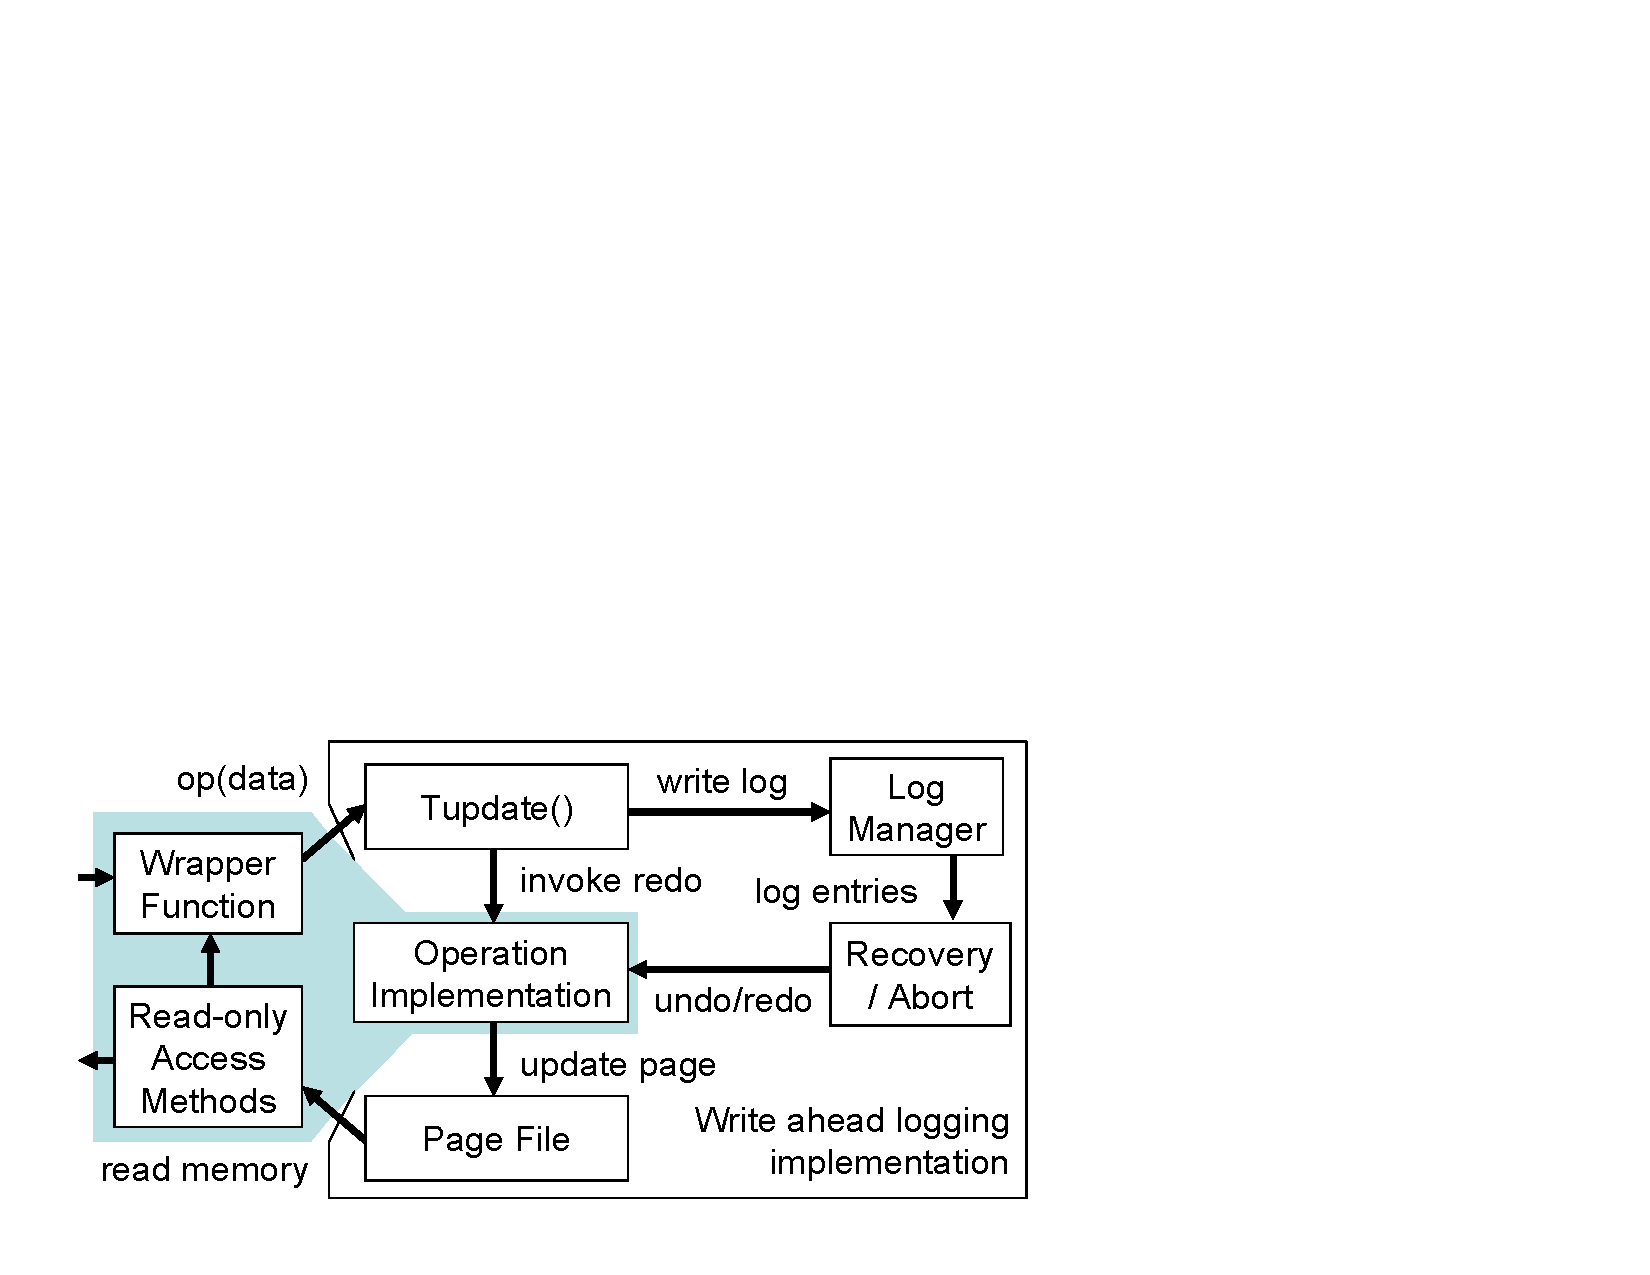
\includegraphics[%
   width=1\columnwidth]{figs/structure.pdf}
\caption{\sf\label{fig:structure} The portions of \yad that directly interact with new operations.}
\end{figure}

The externally visible interface is implemented by wrapper functions
and read-only access methods.  The wrapper function modifies the state
of the page file by packaging the information that will be needed for
undo and redo into a data format of its choosing.  This data structure
is passed into Tupdate().  Tupdate() copies the data to the log, and
then passes the data into the operation's REDO function.
 
REDO modifies the page file directly (or takes some other action).  It
is essentially an interpreter for the log entries it is associated
with.  UNDO works analogously, but is invoked when an operation must
be undone (usually due to an aborted transaction, or during recovery).

This pattern applies in many cases.  In
order to implement a ``typical'' operation, the operation's
implementation must obey a few more invariants:

\begin{itemize}
\item Pages should only be updated inside REDO and UNDO functions.
\item Page updates atomically update the page's LSN by pinning the page.
\item If the data seen by a wrapper function must match data seen
  during REDO, then the wrapper should use a latch to protect against
  concurrent attempts to update the sensitive data (and against
  concurrent attempts to allocate log entries that update the data).
\item Nested top actions (and logical undo) or ``big locks'' (total isolation but lower concurrency) should be used to manage concurrency (Section~\ref{sec:nta}).
\end{itemize}





\section{Experiments}
\label{experiments}

\eab{add transition that explains where we are going}

\subsection{Experimental setup}
\label{sec:experimental_setup}

We chose Berkeley DB in the following experiments because, among
commonly used systems, it provides transactional storage primitives
that are most similar to \yad.  Also, Berkeley DB is 
supported commercially and is designed to provide high performance and high
concurrency.  For all tests, the two libraries provide the same
transactional semantics unless explicitly noted.

All benchmarks were run on an Intel Xeon 2.8 GHz with 1GB of RAM and a
10K RPM SCSI drive formatted using with ReiserFS~\cite{reiserfs}.\endnote{We found that the
  relative performance of Berkeley DB and \yad under single threaded testing is sensitive to
  file system choice, and we plan to investigate the reasons why the
  performance of \yad under ext3 is degraded. However, the results
  relating to the \yad optimizations are consistent across file system
  types.}  All results correspond to the mean of multiple runs with a
95\% confidence interval with a half-width of 5\%.

We used Berkeley DB 4.2.52 as it existed in Debian Linux's testing
branch during March of 2005, with the flags DB\_TXN\_SYNC, and
DB\_THREAD enabled. These flags were chosen to match Berkeley DB's
configuration to \yads as closely as possible.  In cases where
Berkeley DB implements a feature that is not provided by \yad, we
only enable the feature if it improves Berkeley DB's performance.

Optimizations to Berkeley DB that we performed included disabling the
lock manager, though we still use ``Free Threaded'' handles for all
tests.  This yielded a significant increase in performance because it
removed the possibility of transaction deadlock, abort, and
repetition.  However, disabling the lock manager caused highly
concurrent Berkeley DB benchmarks to become unstable, suggesting either a
bug or misuse of the feature.  

With the lock manager enabled, Berkeley
DB's performance in the multithreaded test in Section~\ref{sec:lht} strictly decreased with
increased concurrency.  (The other tests were single-threaded.)  We also
increased Berkeley DB's buffer cache and log buffer sizes to match
\yads default sizes.

We expended a considerable effort tuning Berkeley DB, and our efforts
significantly improved Berkeley DB's performance on these tests.
Although further tuning by Berkeley DB experts would probably improve
Berkeley DB's numbers, we think that we have produced a reasonably
fair comparison.  The results presented here have been reproduced on
multiple machines and file systems.

\subsection{Linear hash table}
\label{sec:lht}

\begin{figure}[t]
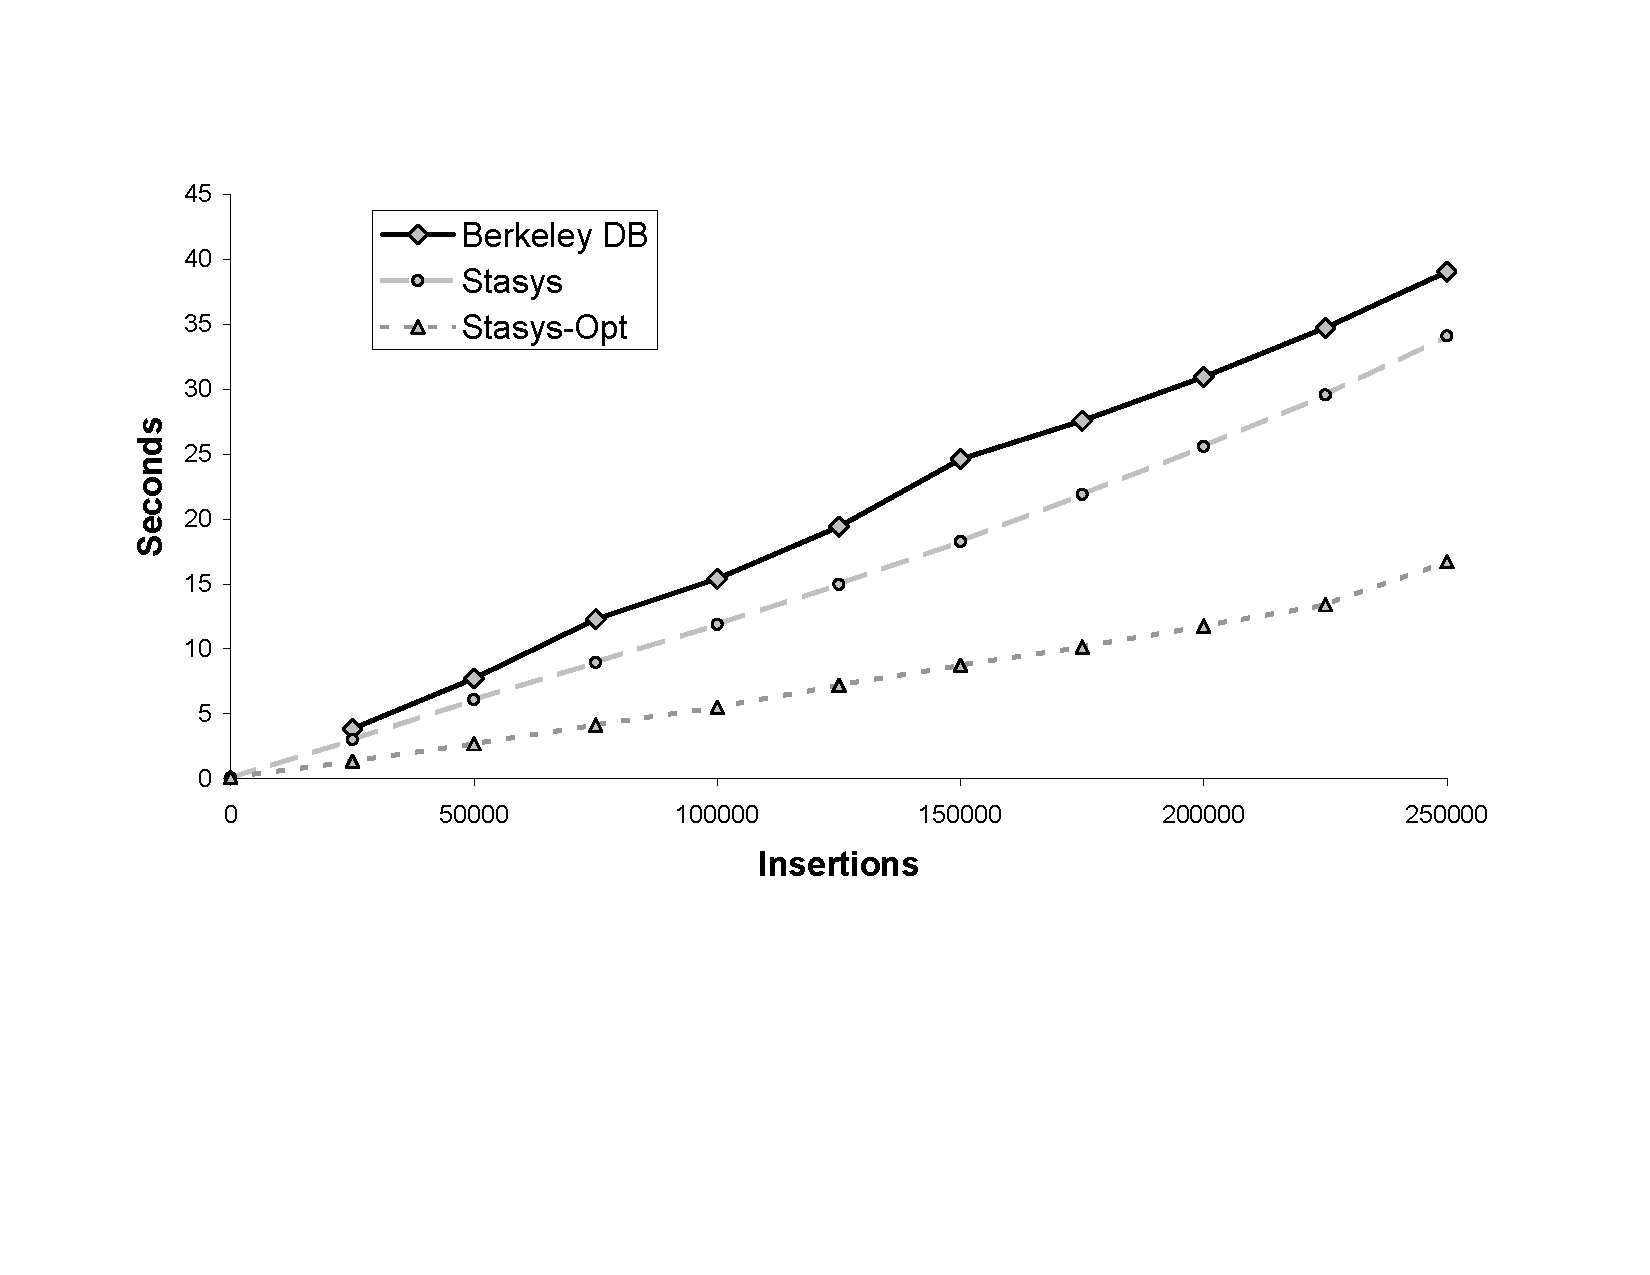
\includegraphics[%
   width=1\columnwidth]{figs/bulk-load.pdf}
%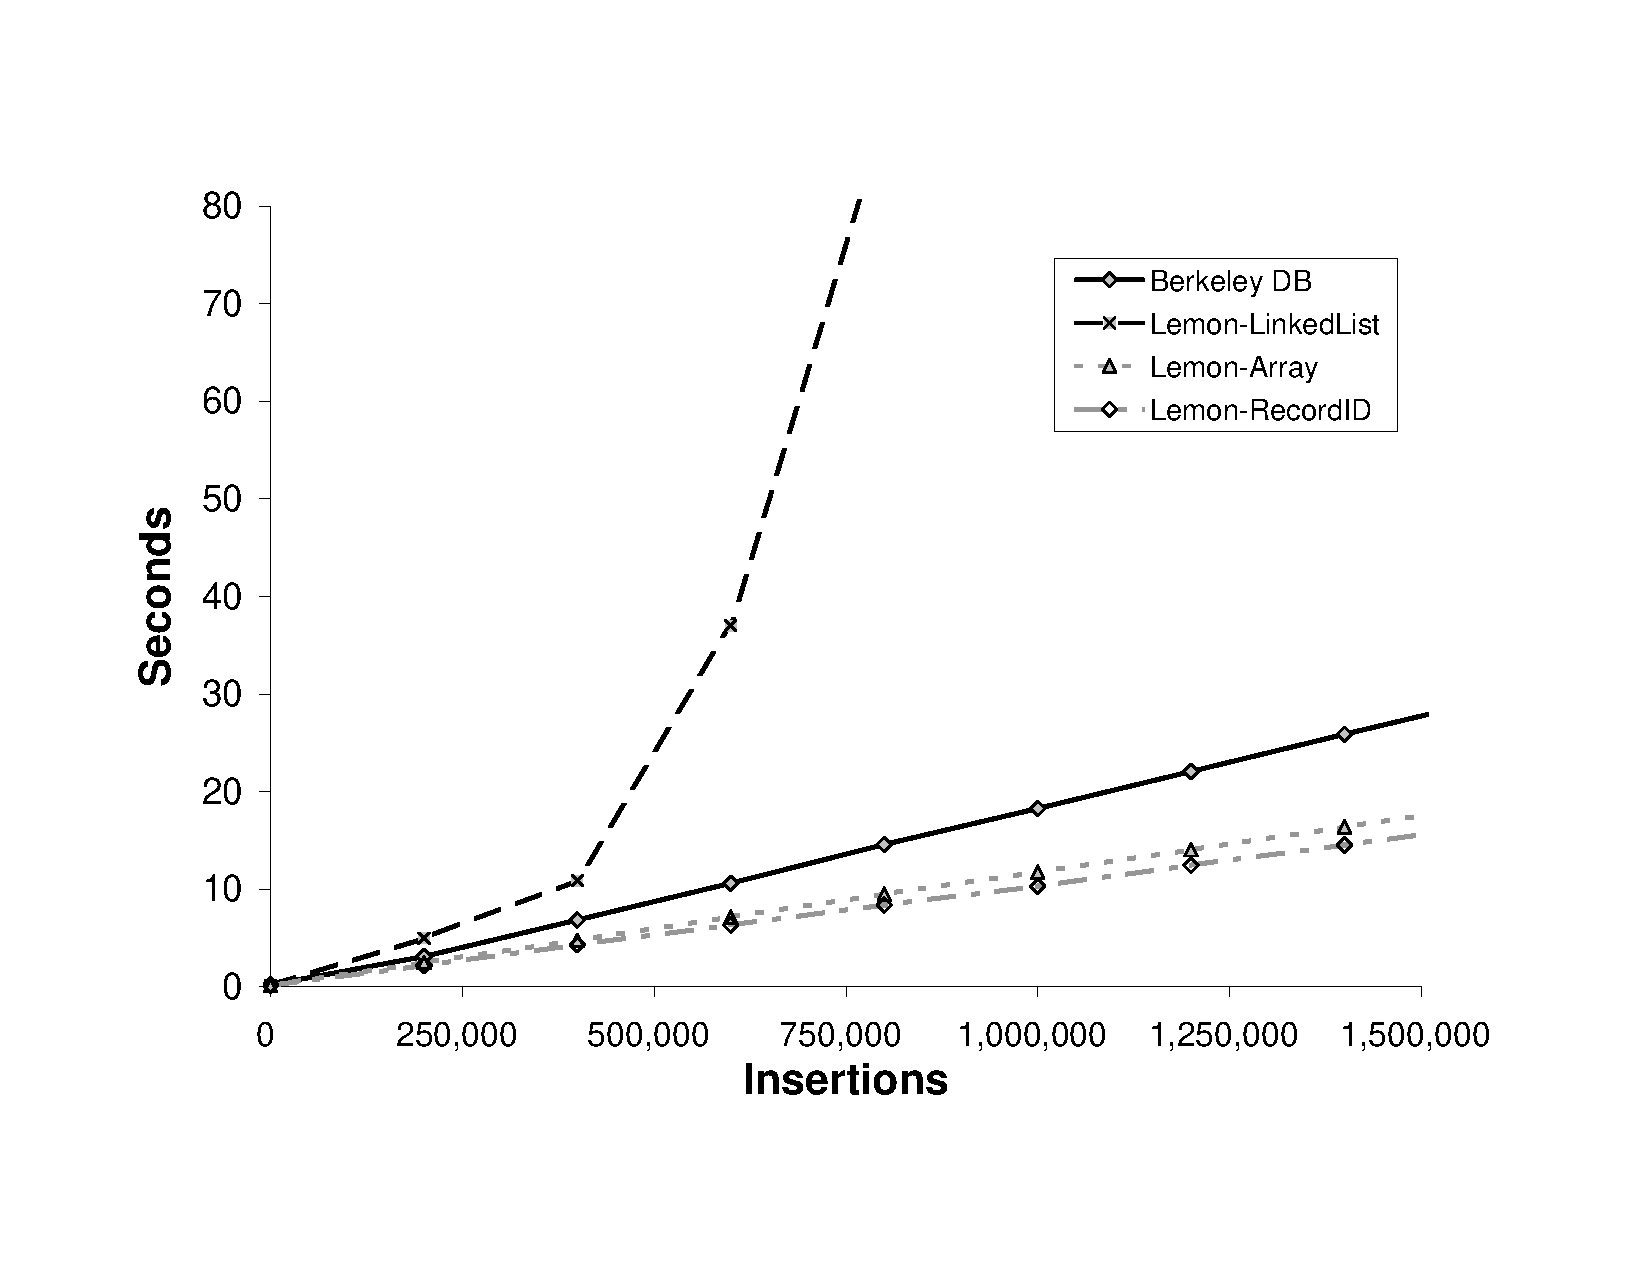
\includegraphics[%
%   width=1\columnwidth]{bulk-load-raw.pdf}
%\vspace{-30pt}
\caption{\sf\label{fig:BULK_LOAD} Performance of \yad and Berkeley DB hash table implementations.  The
test is run as a single transaction, minimizing overheads due to synchronous log writes.}
\end{figure}

\begin{figure}[t]
%\hspace*{18pt}
%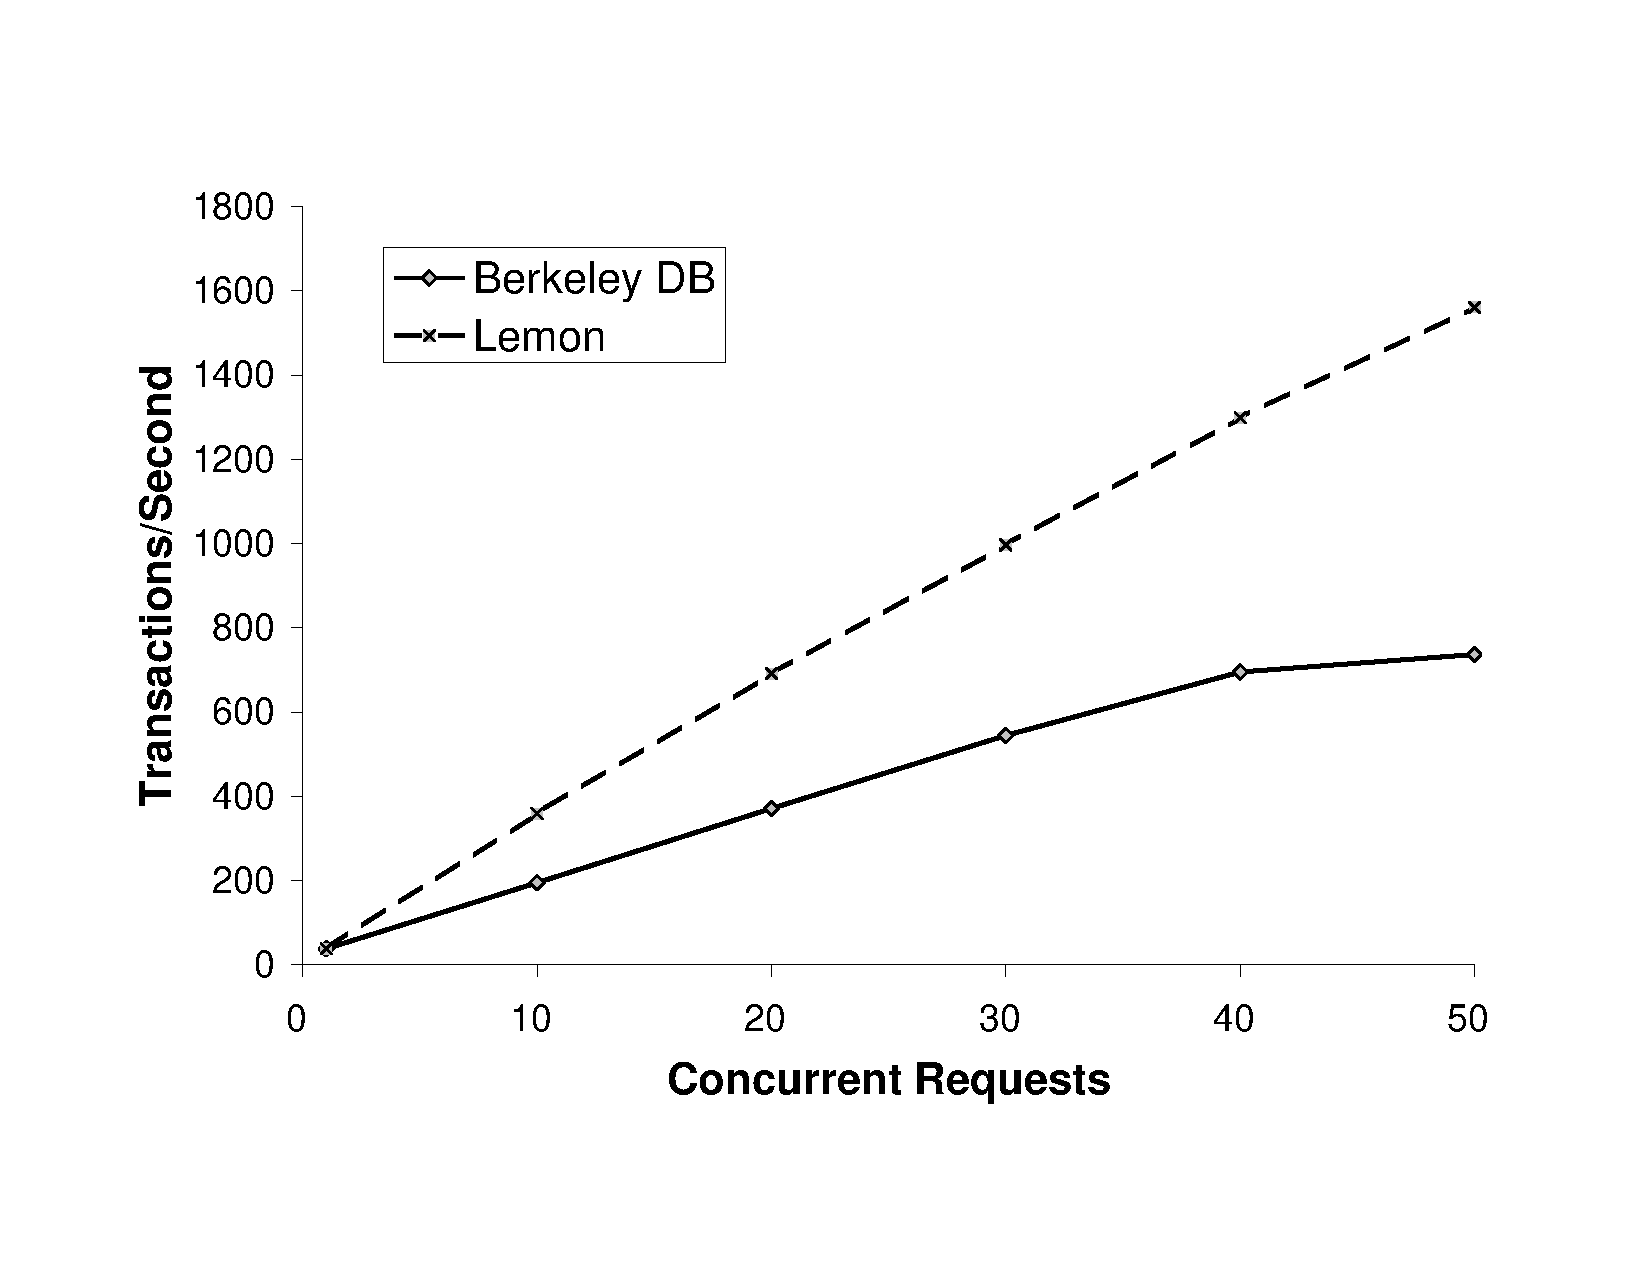
\includegraphics[%
%   width=1\columnwidth]{tps-new.pdf}
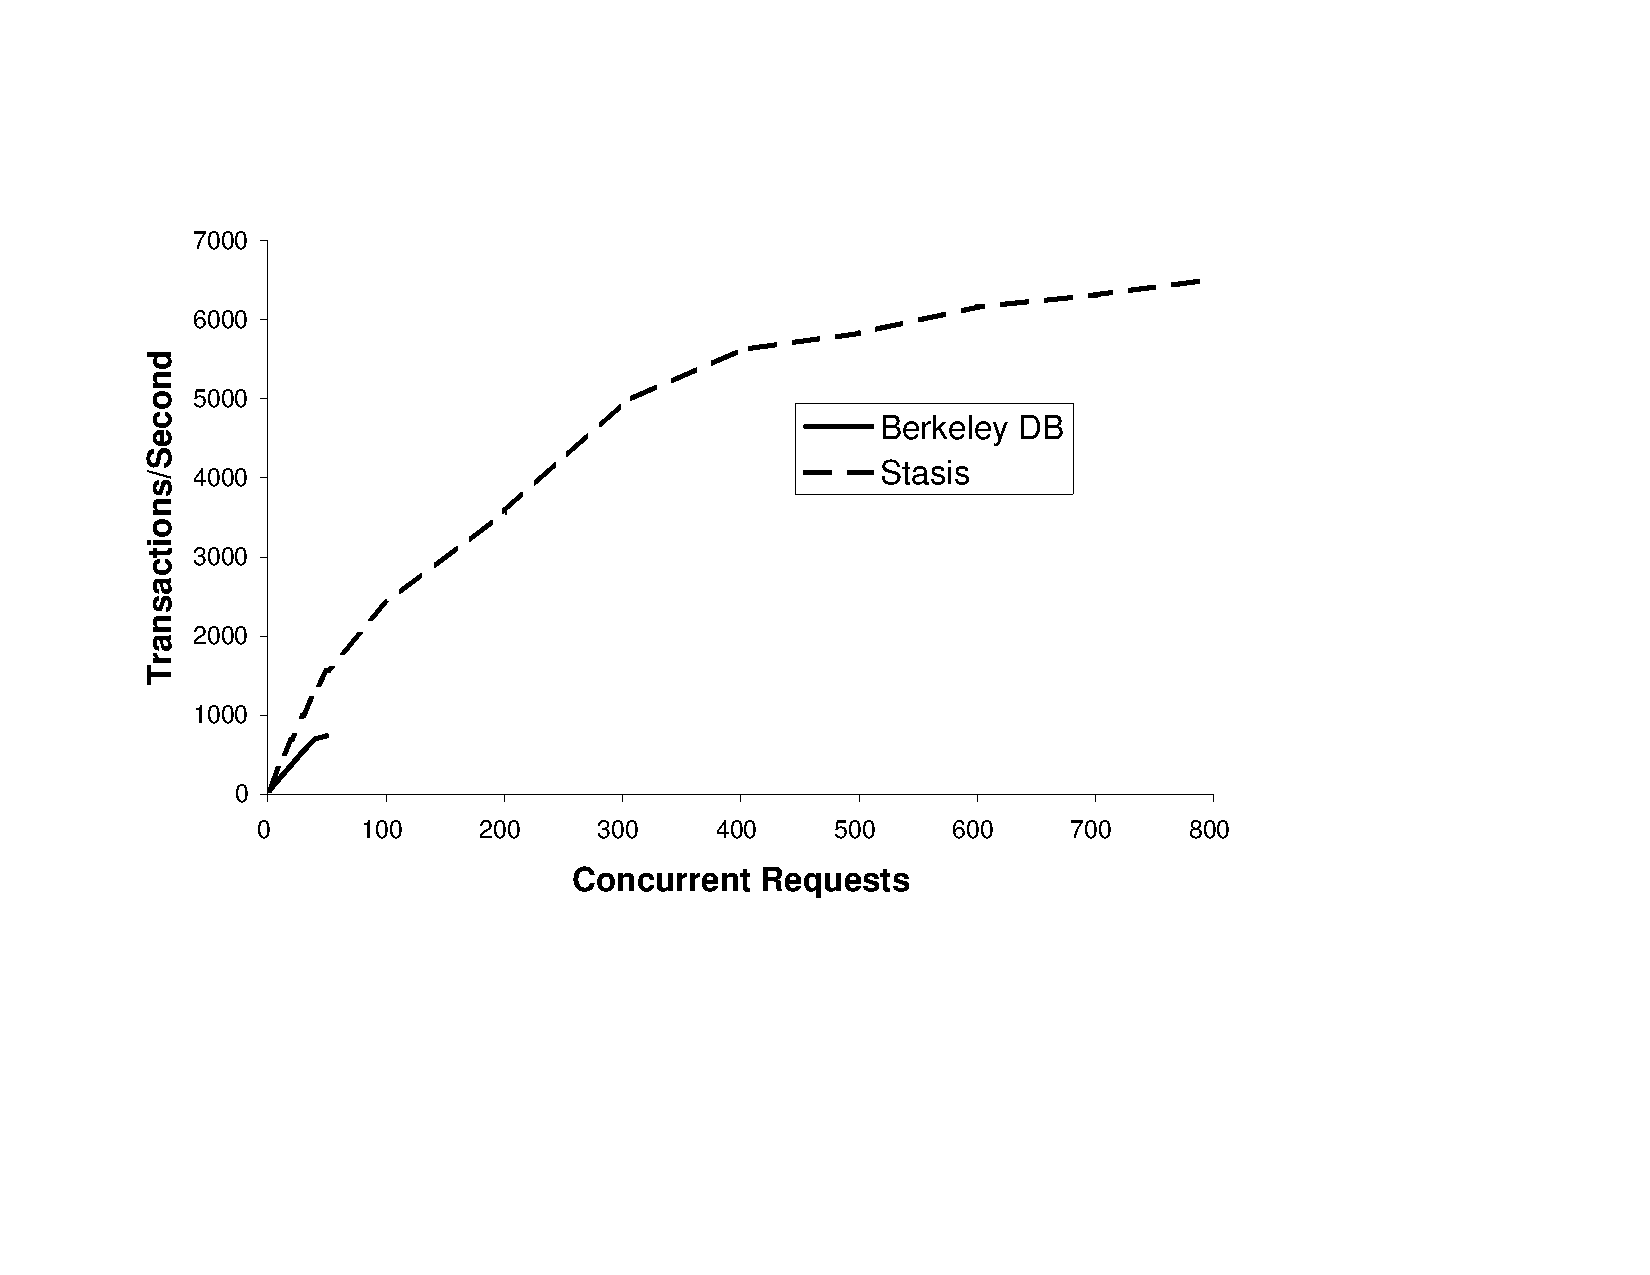
\includegraphics[%
   width=1\columnwidth]{figs/tps-extended.pdf}
%\vspace{-36pt}
\caption{\sf\label{fig:TPS} High concurrency hash table performance of Berkeley DB and \yad.  We were unable to get Berkeley DB to work correctly with more than 50 threads (see text).
}
\end{figure}

Although the beginning of this paper describes the limitations of
physical database models and relational storage systems in great
detail, these systems are the basis of most common transactional
storage routines.  Therefore, we implement a key-based access method
in this section. We argue that obtaining reasonable performance in
such a system under \yad is straightforward.  We then compare our
simple, straightforward implementation to our hand-tuned version and
Berkeley DB's implementation.

The simple hash table uses nested top actions to update its internal
structure atomically.  It uses a {\em linear} hash
function~\cite{lht}, allowing it to increase capacity
 incrementally.  It is based on a number of modular subcomponents.
Notably, its ``table'' is a growable array of fixed-length entries (a
linkset, in the terms of the physical database model) and the user's
choice of two different linked-list implementations. \eab{still
unclear}

The hand-tuned hash table is also built on \yad and also uses a linear hash
function.  However, it is monolithic and uses carefully ordered writes to
reduce runtime overheads such as log bandwidth.  Berkeley DB's
hash table is a popular, commonly deployed implementation, and serves
as a baseline for our experiments.

Both of our hash tables outperform Berkeley DB on a workload that bulk
loads the tables by repeatedly inserting (key, value) pairs
(Figure~\ref{fig:BULK_LOAD}).
%although we do not wish to imply this is always the case.
%We do not claim that our partial implementation of \yad
%generally outperforms, or is a robust alternative
%to Berkeley DB.  Instead, this test shows that \yad is comparable to
%existing systems, and that its modular design does not introduce gross
%inefficiencies at runtime.
The comparison between the \yad  implementations is more
enlightening.  The performance of the simple hash table shows that
straightforward data structure implementations composed from
simpler structures can perform as well as the implementations included 
in existing monolithic systems.  The hand-tuned
implementation shows that \yad allows application developers to
optimize key primitives.

% I cut this because Berkeley db supports custom data structures....

%In the
%best case, past systems allowed application developers to provide
%hints to improve performance.  In the worst case, a developer would be
%forced to redesign and application to avoid sub-optimal properties of
%the transactional data structure implementation.

Figure~\ref{fig:TPS} describes the performance of the two systems under
highly concurrent workloads.  For this test, we used the simple
(unoptimized) hash table, since we are interested in the performance of a
clean, modular data structure that a typical system implementor might
 produce, not the performance of our own highly tuned,
monolithic implementations.

Both Berkeley DB and \yad can service concurrent calls to commit with
a single synchronous I/O.\endnote{The multi-threaded benchmarks
  presented here were performed using an ext3 file system, as high
  concurrency caused both Berkeley DB and \yad to behave unpredictably
  when ReiserFS was used.  However, \yads multi-threaded throughput
  was significantly better that Berkeley DB's under both file systems.}
\yad scaled quite well, delivering over 6000 transactions per
second,\endnote{The concurrency test was run without lock managers, and the
  transactions obeyed the A, C, and D properties.  Since each
  transaction performed exactly one hash table write and no reads, they also
  obeyed I (isolation) in a trivial sense.}  and provided roughly
double Berkeley DB's throughput (up to 50 threads).  Although not
shown here, we found that the latencies of Berkeley DB and \yad were
similar, which confirms that \yad is not simply trading latency for
throughput during the concurrency benchmark.


\begin{figure*}
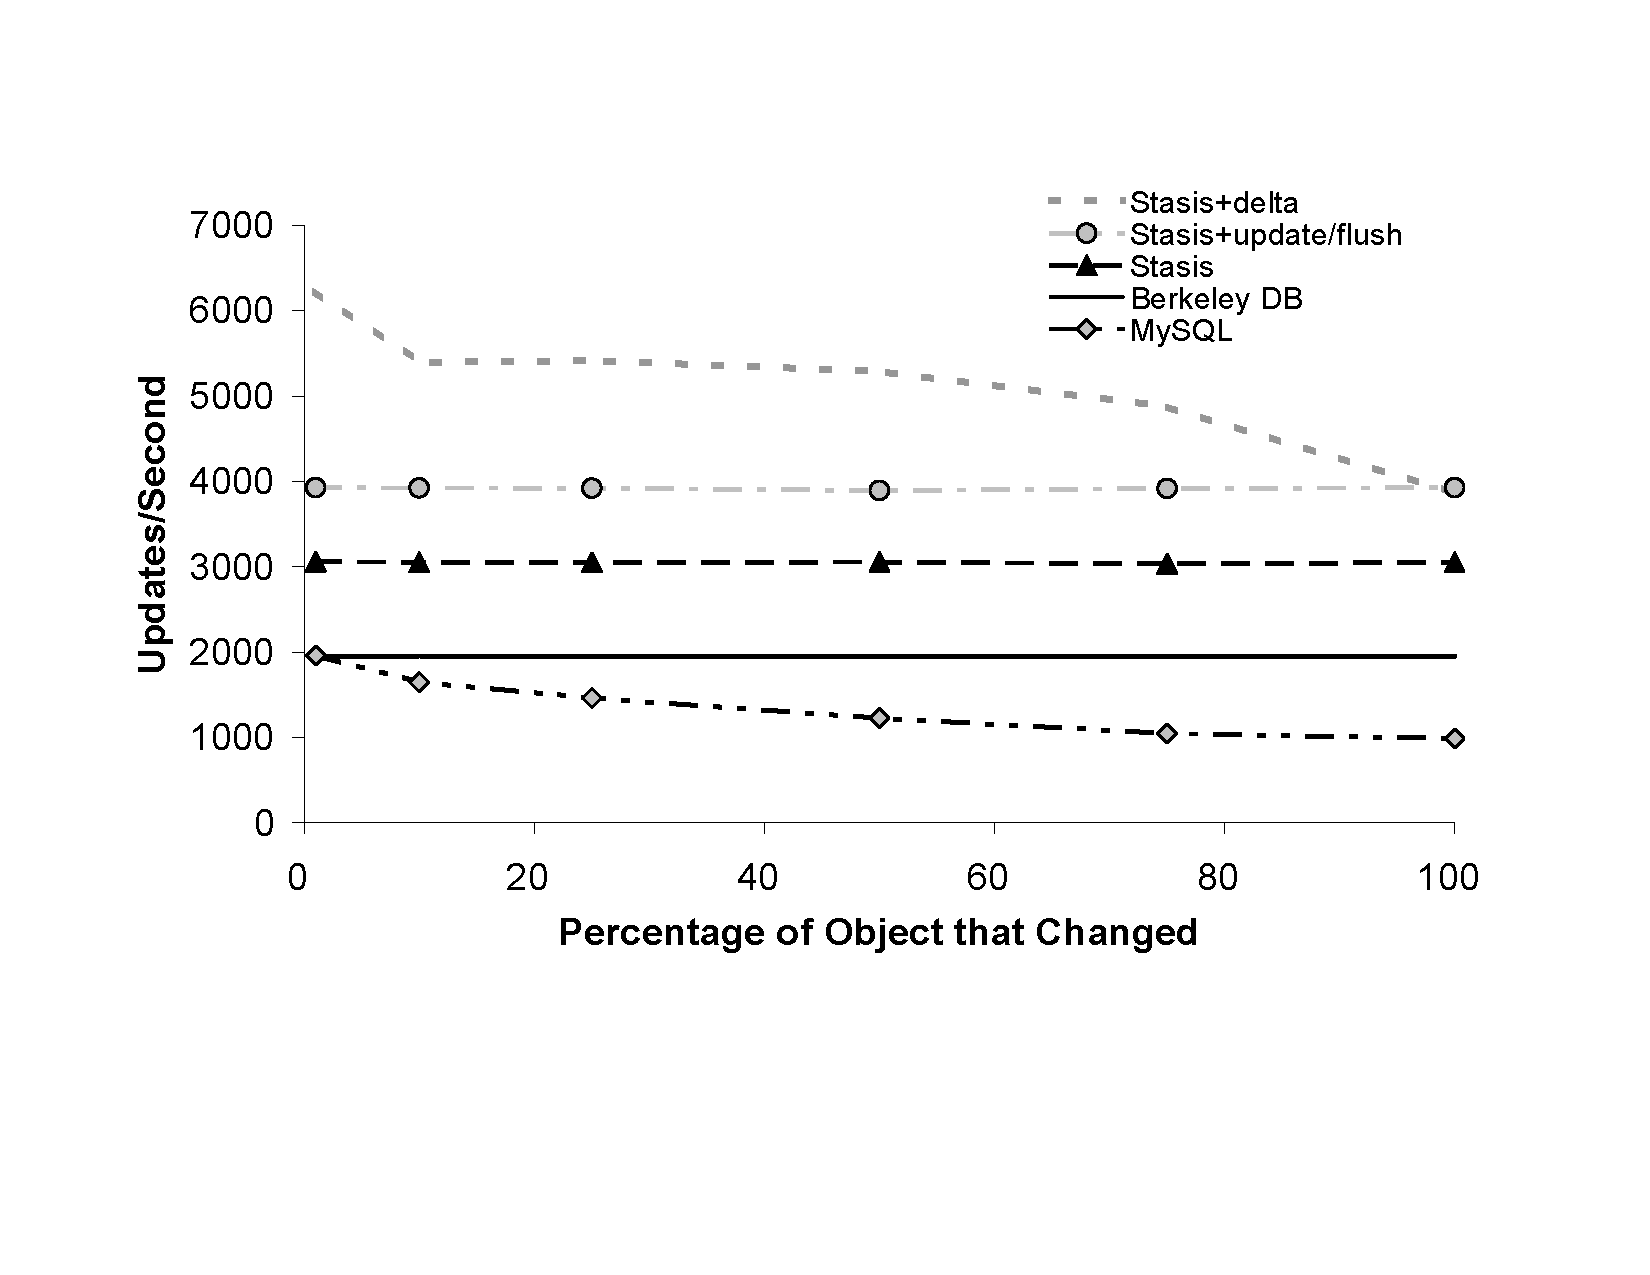
\includegraphics[width=1\columnwidth]{figs/object-diff.pdf}
\hspace{.2in}
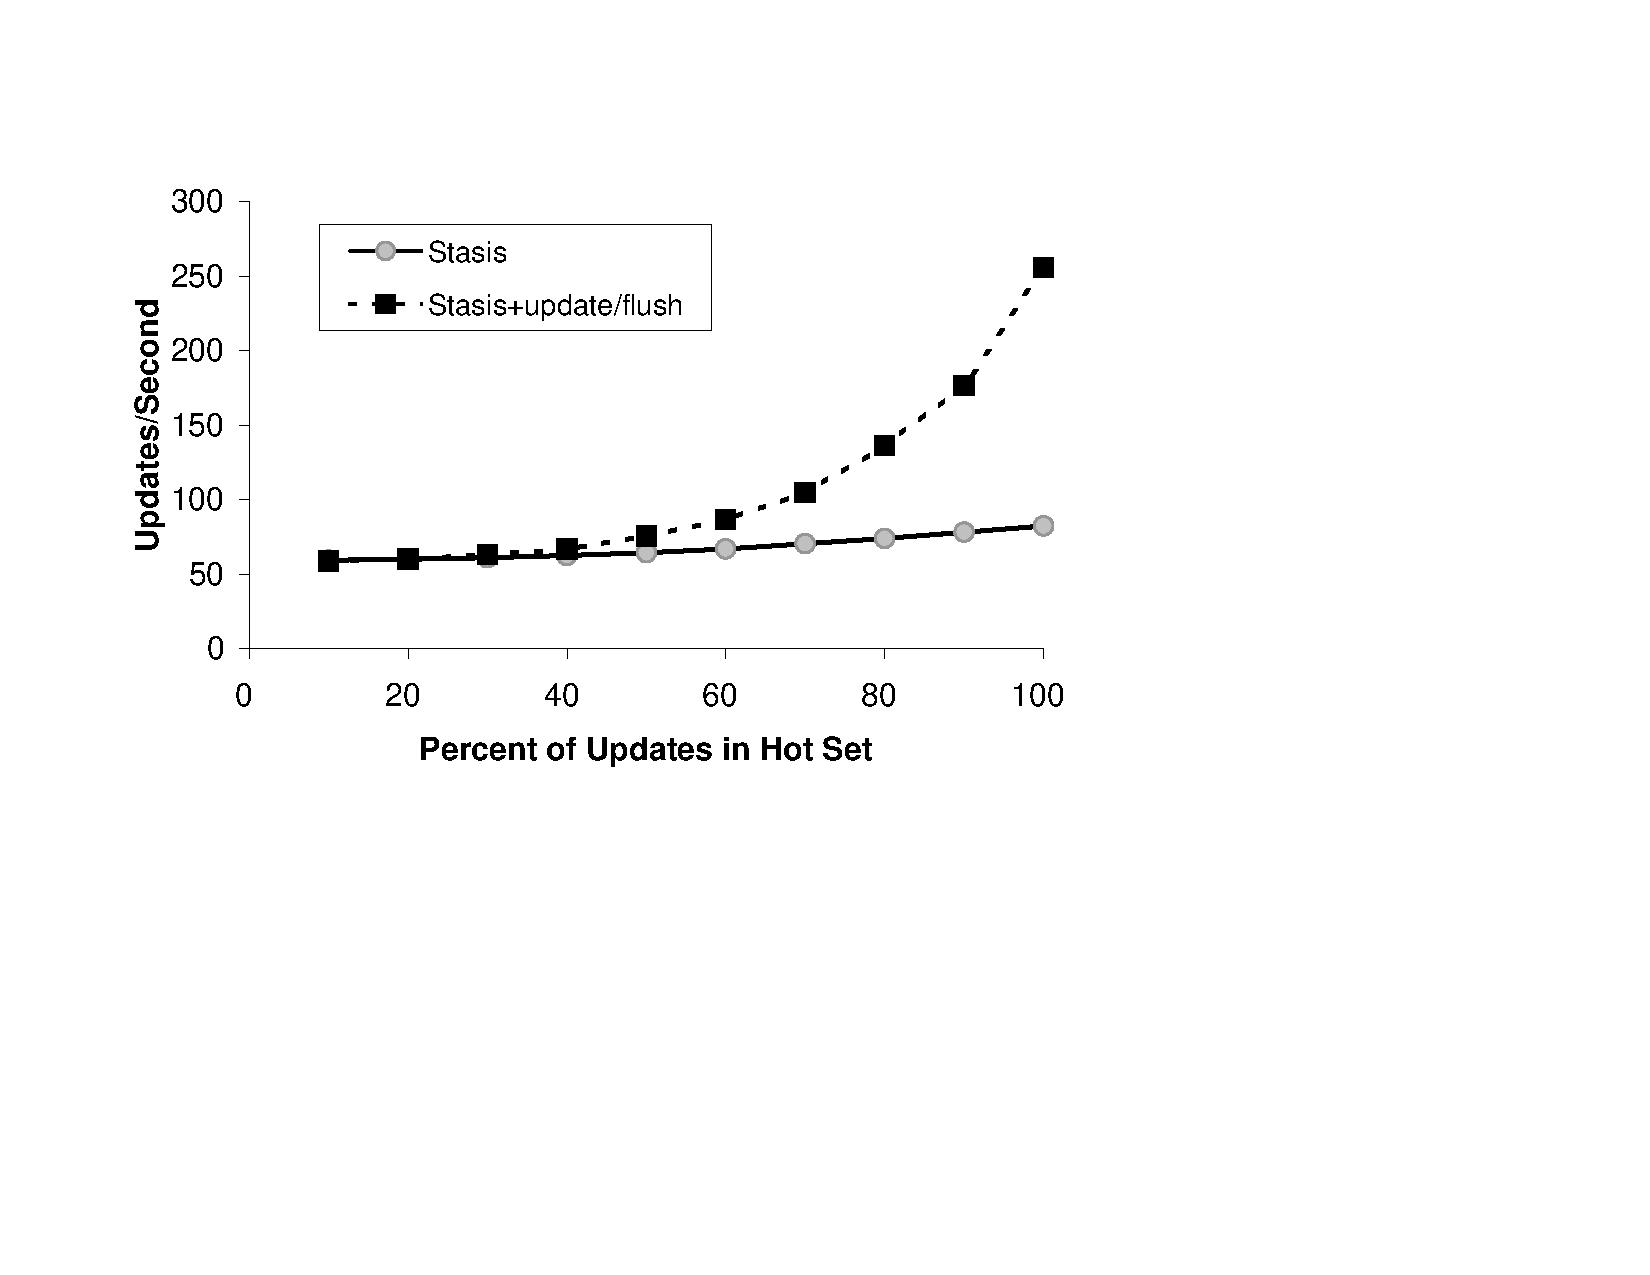
\includegraphics[width=1\columnwidth]{figs/mem-pressure.pdf}
\vspace{-.15in}
\caption{\sf \label{fig:OASYS}
The effect of \yad object serialization optimizations under low and high memory pressure.}
\end{figure*}


\subsection{Object persistence}
\label{sec:oasys}

Numerous schemes are used for object serialization.  Support for two
different styles of object serialization has been implemented in
\yad.  We could have just as easily implemented a persistence
mechanism for a statically typed functional programming language, a
dynamically typed scripting language, or a particular application,
such as an email server.  In each case, \yads lack of a hard-coded data
model would allow us to choose the representation and transactional
semantics that make the most sense for the system at hand.

The first object persistence mechanism, pobj, provides transactional updates to objects in
Titanium, a Java variant.  It transparently loads and persists
entire graphs of objects, but will not be discussed in further detail.

The second variant was built on top of a C++ object
serialization library, \oasys.  \oasys makes use of pluggable storage
modules that implement persistent storage, and includes plugins
for Berkeley DB and MySQL.  

This section will describe how the \yad \oasys plugin reduces the
amount of data written to log, while using half as much system memory
as the other two systems.

We present three variants of the \yad plugin here.  The first treats
\yad like Berkeley DB.  The second, the ``update/flush'' variant
customizes the behavior of the buffer manager, and the third,
``delta'', extends the second wiht support for logging only the deltas
between versions.

The update/flush variant avoids maintaining an up-to-date
version of each object in the buffer manager or page file: it allows
the buffer manager's view of live application objects to become stale.
This is safe since the system is always able to reconstruct the
appropriate page entry from the live copy of the object.

By allowing the buffer manager to contain stale data, we reduce the
number of times the \yad \oasys plugin must update serialized objects in the buffer manager.
%  Reducing the number of serializations decreases
%CPU utilization, and it also
This allows us to drastically decrease the
size of the page file.  In turn this allows us to increase the size of
the application's cache of live objects.

We implemented the \yad buffer-pool optimization by adding two new
operations, update(), which only updates the log, and flush(), which
updates the page file.  

The reason it would be difficult to do this with Berkeley DB is that
we still need to generate log entries as the object is being updated.
  This would cause Berkeley DB to write data back to the page file,
increasing the working set of the program, and increasing disk
activity.

Furthermore, objects may be written to disk in an
order that differs from the order in which they were updated, 
violating one of the write-ahead logging invariants.  One way to 
deal with this is to maintain multiple LSNs per page.  This means we would need to register a
callback with the recovery routine to process the LSNs (a similar
callback will be needed in Section~\ref{sec:zeroCopy}), and 
extend \yads page format to contain per-record LSNs.  
Also, we must prevent \yads storage allocation routine from overwriting the per-object 
LSNs of deleted objects that may still be addressed during abort or recovery.\eab{tombstones discussion here?}  

\eab{we should at least implement this callback if we have not already}

Alternatively, we could arrange for the object pool to cooperate 
further with the buffer pool by atomically updating the buffer 
manager's copy of all objects that share a given page, removing the 
need for multiple LSNs per page, and simplifying storage allocation.

However, the simplest solution, and the one we take here, is based on
the observation that updates (not allocations or deletions) of
fixed-length objects are blind writes.  This allows us to do away with
per-object LSNs entirely.  Allocation and deletion can then be
handled as updates to normal LSN containing pages.  At recovery time,
object updates are executed based on the existence of the object on
the page and a conservative estimate of its LSN.  (If the page doesn't
contain the object during REDO then it must have been written back to
disk after the object was deleted.  Therefore, we do not need to apply
the REDO.)  This means that the system can ``forget'' about objects
that were freed by committed transactions, simplifying space reuse
tremendously.  (Because LSN-free pages and recovery are not yet
implemented, this benchmark mimics their behavior at runtime, but does
not support recovery.)

The third plugin variant, ``delta'', incorporates the update/flush
optimizations, but only writes the changed portions of
objects to the log.  Because of \yads support for custom log-entry
formats, this optimization is straightforward.

%In addition to the buffer-pool optimizations, \yad provides several 
%options to handle UNDO records in the context
%of object serialization. The first is to use a single transaction for
%each object modification, avoiding the cost of generating or logging
%any UNDO records. The second option is to assume that the
%application will provide a custom UNDO for the delta, 
%which increases the size of the log entry generated by each update, 
%but still avoids the need to read or update the page
%file.
%
%The third option is to relax the atomicity requirements for a set of
%object updates and again avoid generating any UNDO records. This
%assumes that the application cannot abort individual updates, 
%and is willing to
%accept that some prefix of logged but uncommitted updates may 
%be applied to the page
%file after recovery. 

\oasys does not export transactions to its callers.  Instead, it
is designed to be used in systems that stream objects over an
unreliable network connection.  Each object update corresponds to an
independent message, so there is never any reason to roll back an
applied object update.  On the other hand, \oasys does support a
flush method, which guarantees the durability of updates after it
returns.  In order to match these semantics as closely as possible,
\yads update/flush and delta optimizations do not write any 
undo information to the log.  

These ``transactions'' are still durable
after commit, as commit forces the log to disk. 
%For the benchmarks below, we
%use this approach, as it is the most aggressive and is
As far as we can tell, MySQL and Berkeley DB do not support this
optimization in a straightforward fashion.  (``Auto-commit'' comes
close, but does not quite provide the correct durability semantics.)
%not supported by any other general-purpose transactional 
%storage system (that we know of).

The operations required for these two optimizations required 
150 lines of C code, including whitespace, comments and boilerplate
function registrations.\endnote{These figures do not include the
  simple LSN-free object logic required for recovery, as \yad does not
  yet support LSN-free operations.}  Although the reasoning required
to ensure the correctness of this code is complex, the simplicity of
the implementation is encouraging.

In this experiment, Berkeley DB was configured as described above.  We
ran MySQL using InnoDB for the table engine.  For this benchmark, it
is the fastest engine that provides similar durability to \yad. We
linked the benchmark's executable to the libmysqld daemon library,
bypassing the RPC layer. In experiments that used the RPC layer, test
completion times were orders of magnitude slower.

Figure~\ref{fig:OASYS} presents the performance of the three
\yad optimizations, and the \oasys plugins implemented on top of other
systems.  As we can see, \yad performs better than the baseline
systems, which is not surprising, since it is not providing the A
property of ACID transactions.  (Although it is applying each individual operation atomically.)

In non-memory bound systems, the optimizations nearly double \yads
performance by reducing the CPU overhead of object serialization and
the number of log entries written to disk.  In the memory bound test,
we see that update/flush indeed improves memory utilization.


\subsection{Manipulation of logical log entries}

\eab{this section unclear, including title}

\label{sec:logging}
\begin{figure}
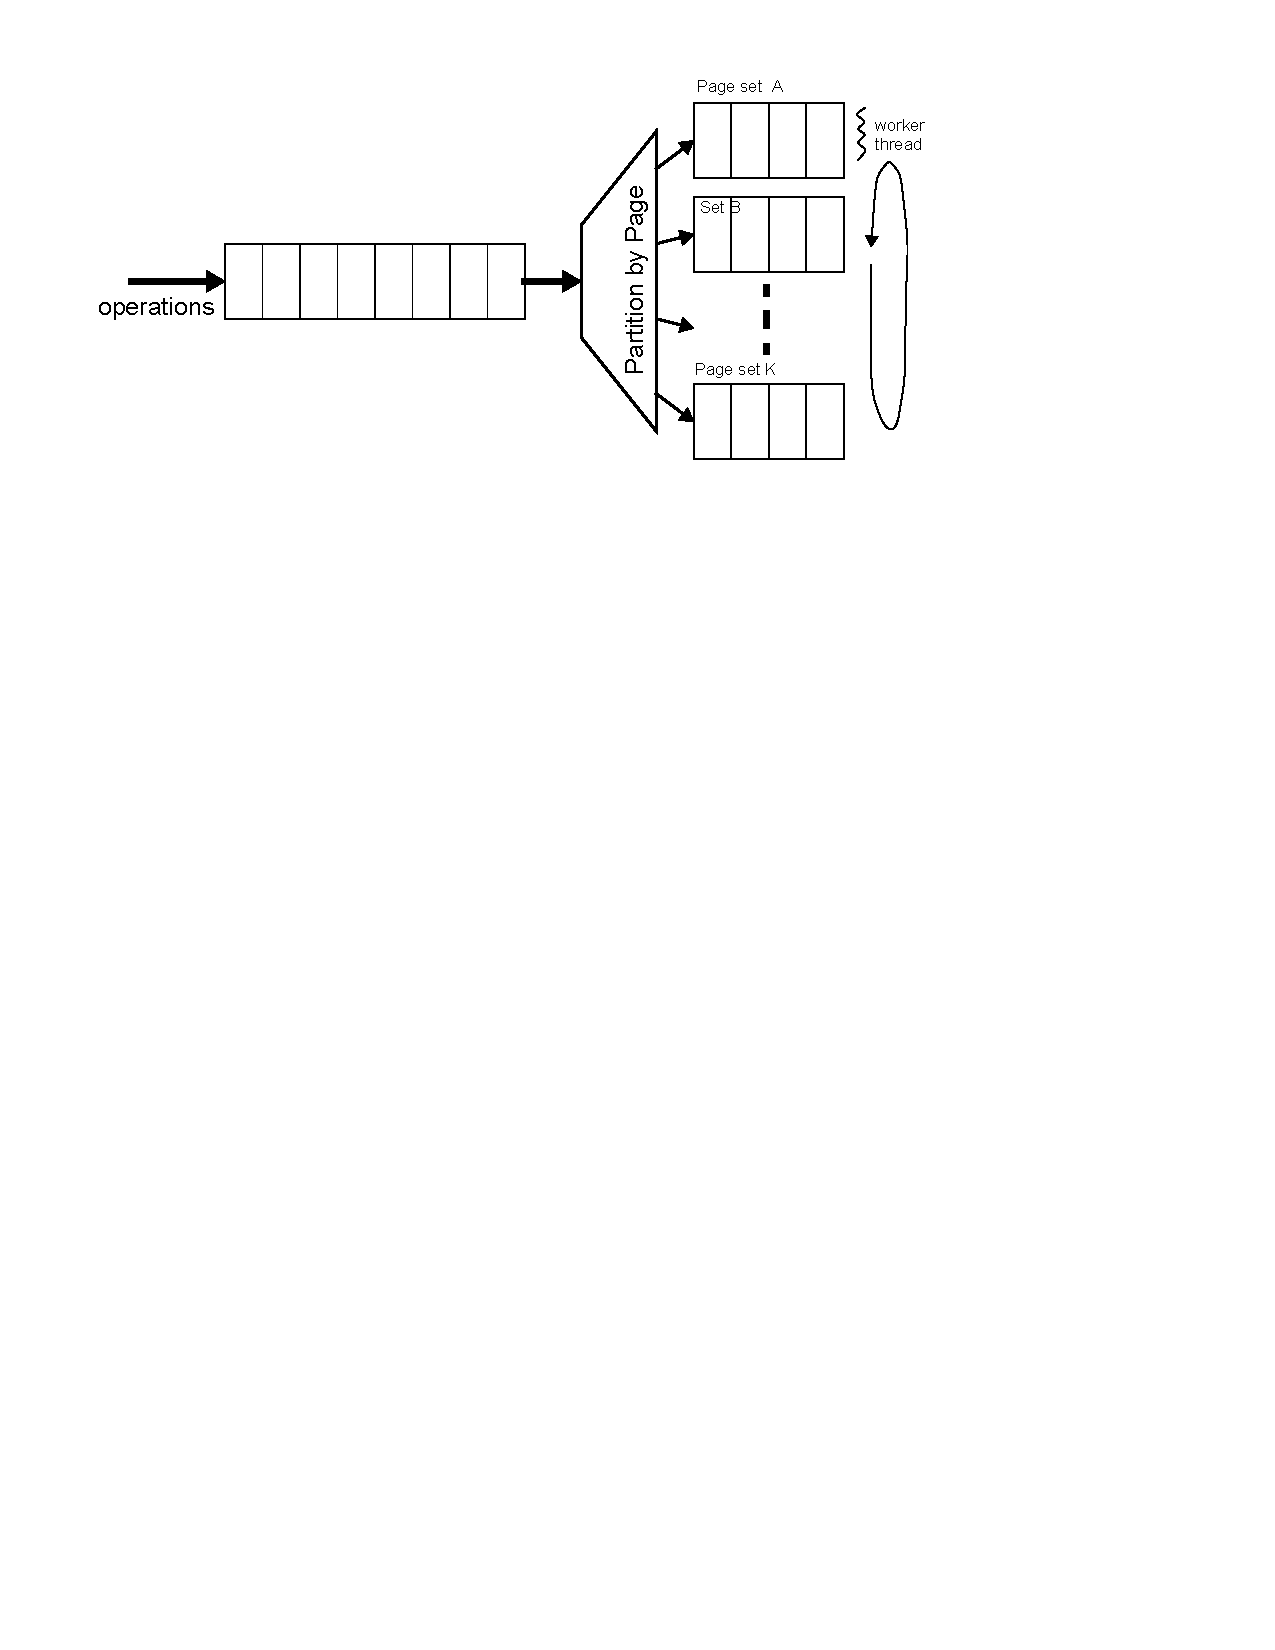
\includegraphics[width=1\columnwidth]{figs/graph-traversal.pdf}
\vspace{-24pt}
\caption{\sf\label{fig:multiplexor} Because pages are independent, we
can reorder requests among different pages. Using a log demultiplexer,
we partition requests into independent queues, which can be 
handled in any order, improving locality and merging opportunities.}
\end{figure}
\begin{figure}[t]
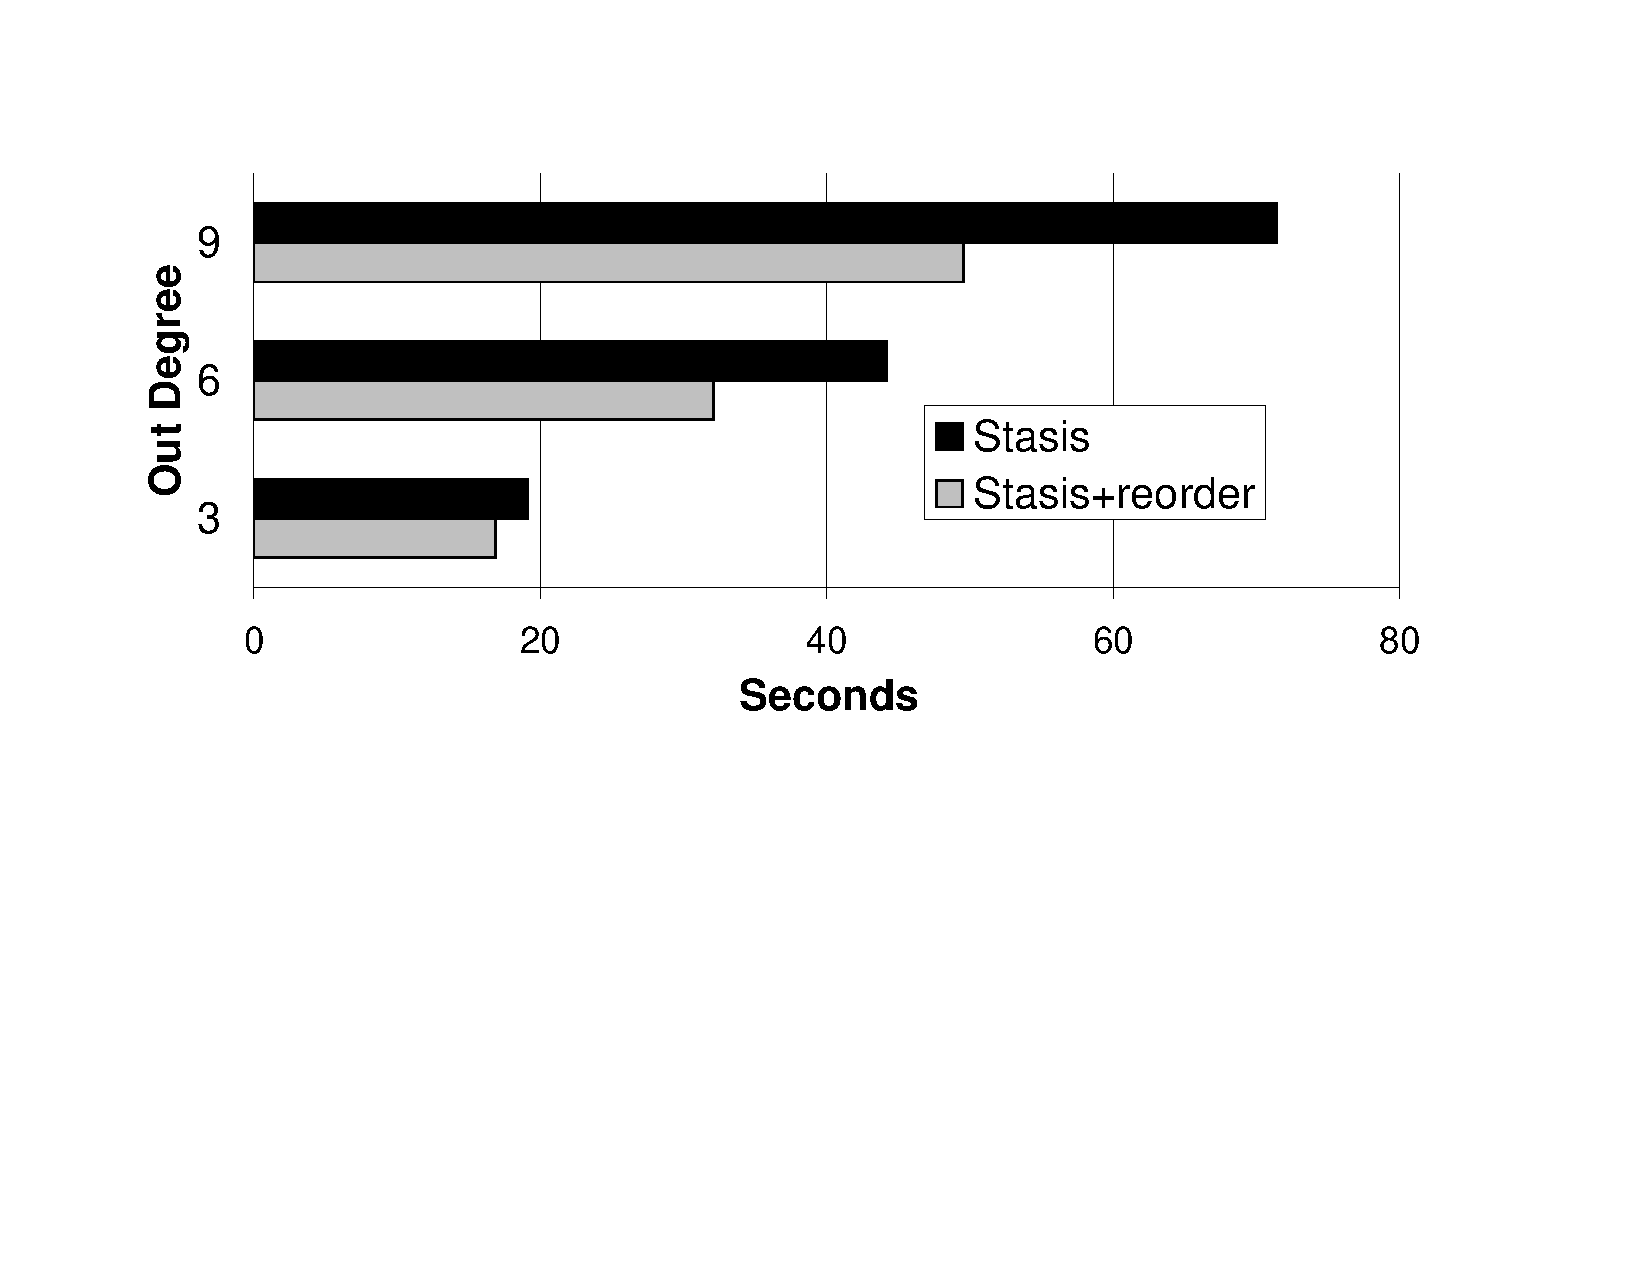
\includegraphics[width=1\columnwidth]{figs/oo7.pdf}
\vspace{-15pt}
\caption{\sf\label{fig:oo7} OO7 benchmark style graph traversal.  The optimization performs well due to the presence of non-local nodes.}
\end{figure}

\begin{figure}[t]
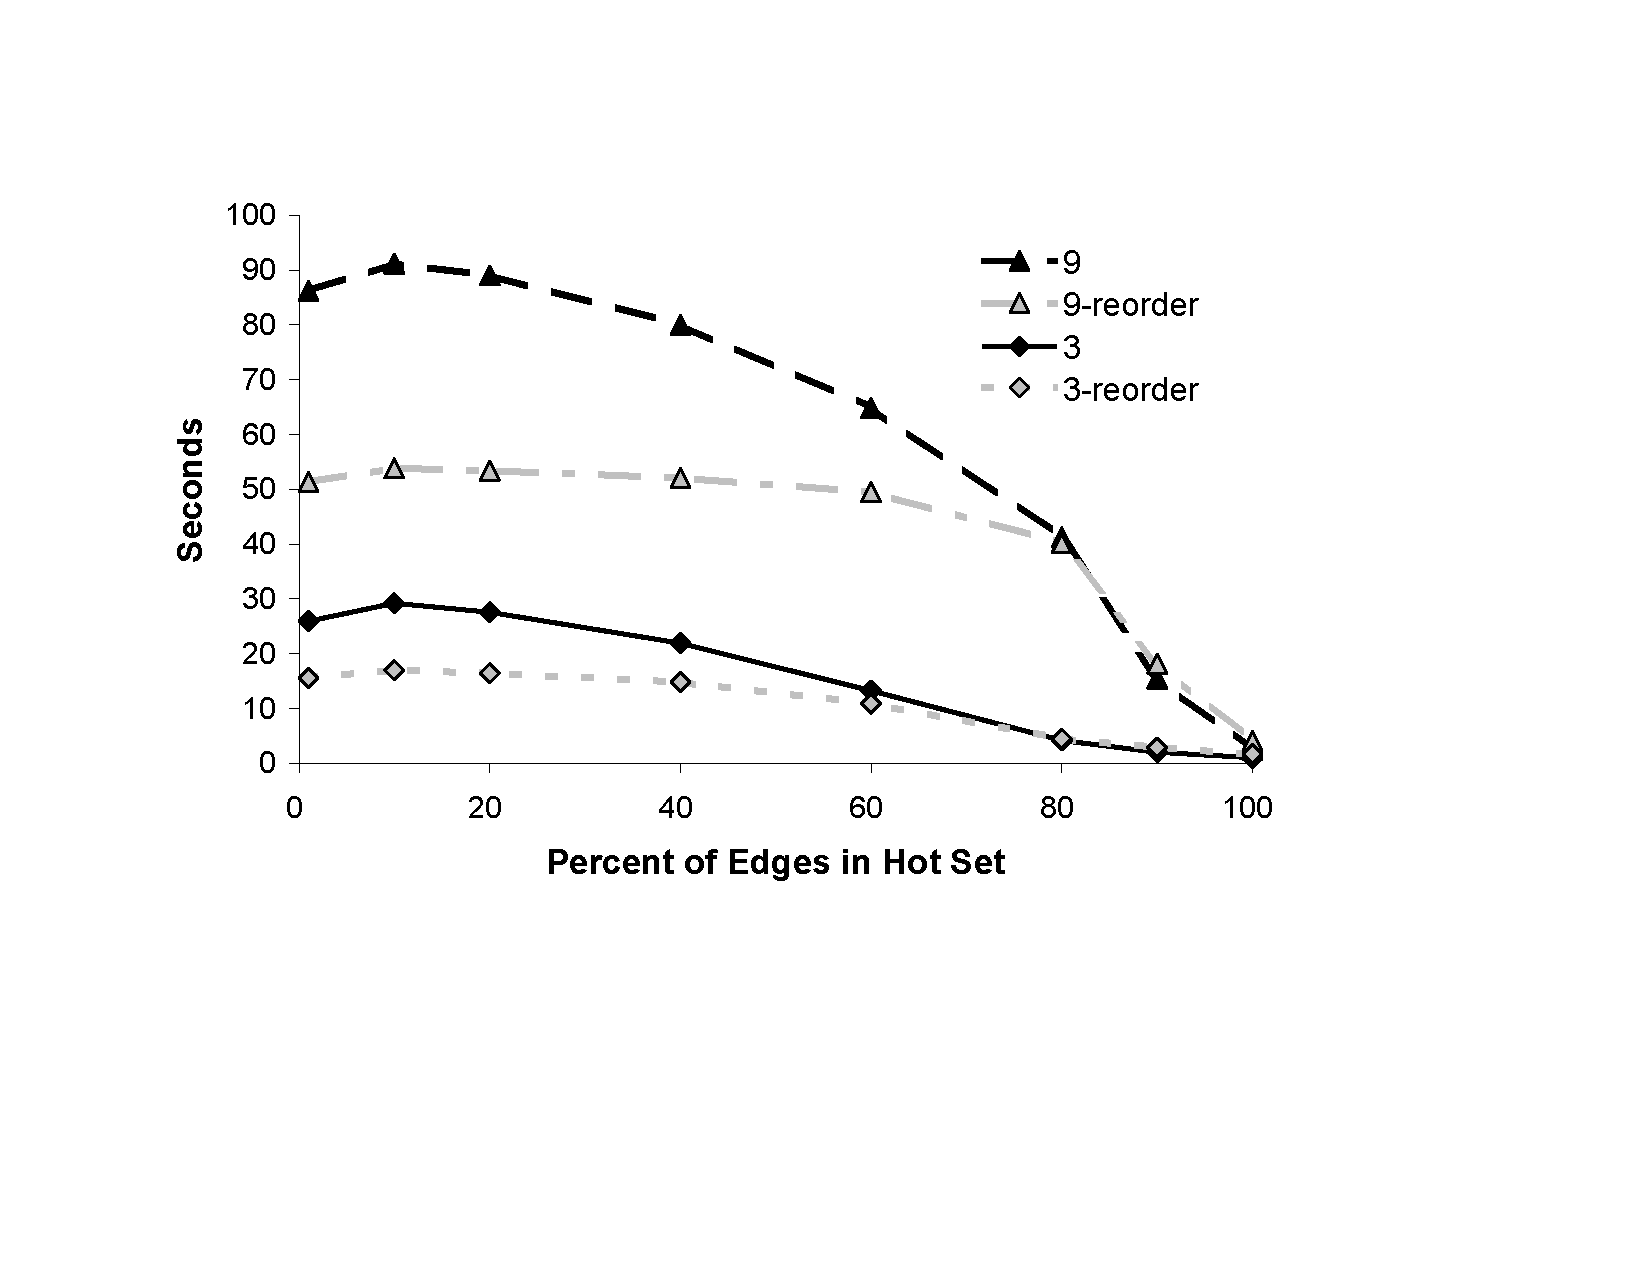
\includegraphics[width=1\columnwidth]{figs/trans-closure-hotset.pdf}
\vspace{-12pt}
\caption{\sf\label{fig:hotGraph} Hot set based graph traversal for random graphs with out-degrees of 3 and 9.  Here
we see that the multiplexer helps when the graph has poor locality.
In the cases where depth first search performs well, the
reordering is inexpensive.}
\end{figure}

Database optimizers operate over relational algebra expressions that
correspond to logical operations over streams of data.  \yad
does not provide query languages, relational algebra, or other such query processing primitives.  

However, it does include an extensible logging infrastructure.
Furthermore, \diff{most operations that support concurrent transactions already
provide logical UNDO (and therefore logical REDO, if each operation has an
inverse).}
%many
%operations that make use of physiological logging implicitly
%implement UNDO (and often REDO) functions that interpret logical
%requests.

Logical operations often have some nice properties that this section
will exploit.  Because they can be invoked at arbitrary times in the
future, they tend to be independent of the database's physical state.
Often, they correspond to operations that programmers understand.

Because of this, application developers can easily determine whether
logical operations may be reordered, transformed, or even
dropped from the stream of requests that \yad is processing.

If requests can be partitioned in a natural way, load
balancing can be implemented by splitting requests across many nodes.
Similarly, a node can easily service streams of requests from multiple
nodes by combining them into a single log, and processing the log
using operation implementations.  For example, this type of optimization 
is used by RVM's log-merging operations~\cite{lrvm}.

Furthermore, application-specific
procedures that are analogous to standard relational algebra methods
(join, project and select) could be used to efficiently transform the data
while it is still laid out sequentially
in non-transactional memory.

%Note that read-only operations do not necessarily generate log
%entries.  Therefore, applications may need to implement custom
%operations to make use of the ideas in this section.

Therefore, we implemented a single node log-reordering scheme that increases request locality
during the traversal of a random graph.  The graph traversal system
takes a sequence of (read) requests, and partitions them using some
function.  It then processes each partition in isolation from the
others.  We considered two partitioning functions.  The first divides the page file
into equally sized contiguous regions, which increases locality.  The second takes the hash
of the page's offset in the file, which enables load balancing.
%%  The second policy is interesting
%The first, partitions the
%requests according to the hash of the node id they refer to, and would be useful for load balancing over a network.
%(We expect the early phases of such a traversal to be bandwidth, not
%latency limited, as each node would stream large sequences of
%asynchronous requests to the other nodes.) 

Our benchmarks partition requests by location.  We chose the
position size so that each partition can fit in \yads buffer pool.

We ran two experiments.  Both stored a graph of fixed size objects in
the growable array implementation that is used as our linear
hash table's bucket list.
The first experiment (Figure~\ref{fig:oo7})
is loosely based on the OO7 database benchmark~\cite{oo7}.  We
hard-code the out-degree of each node, and use a directed graph.  OO7
constructs graphs by first connecting nodes together into a ring.
It then randomly adds edges between the nodes until the desired
out-degree is obtained.  This structure ensures graph connectivity.
If the nodes are laid out in ring order on disk then it also ensures that
one edge from each node has good locality, while the others generally
have poor locality.

The second experiment explicitly measures the effect of graph locality
on our optimization (Figure~\ref{fig:hotGraph}). It extends the idea
of a hot set to graph generation.  Each node has a distinct hot set
that includes the 10\% of the nodes that are closest to it in ring
order.  The remaining nodes are in the cold set.  We use random edges
instead of ring edges for this test.  This does not ensure graph
connectivity, but we used the same random seeds for the two systems.

When the graph has good locality, a normal depth first search
traversal and the prioritized traversal both perform well.  The
prioritized traversal is slightly slower due to the overhead of extra
log manipulation. As locality decreases, the partitioned traversal
algorithm's outperforms the naive traversal.


\section{Related Work}
\label{related-work}


\eab{moved text here from section 2 to make it smaller and less technical}

\subsection{Database Variations} 
\label{sec:otherDBs}

This section discusses transaction systems with goals
similar to ours.  Although these projects were successful in many
respects, they fundamentally aimed to extend the range of their
abstract data model, which in the end still has limited overall range.
In contrast, \yad follows a bottom-up approach that enables can
implement (in theory) any of these abstract models and their extensions.

\subsubsection{Extensible databases}

Genesis~\cite{genesis}, an early database toolkit, was built in terms
of a physical data model and the conceptual mappings described above. \rcs{I think they say this is an explicit design choice.}
It is designed to allow database implementors to easily swap out
implementations of the various components defined by its framework.
Like subsequent systems (including \yad), it allows its users to
implement custom operations.

Subsequent extensible database work builds upon these foundations.
The Exodus~\cite{exodus} database toolkit is the successor to
Genesis. It supports the automatic generation of query optimizers and
execution engines based upon abstract data type definitions, access
methods and cost models provided by its users.

Although further discussion is beyond the scope of this paper,
object-oriented database systems (\rcs{cite something?}) and relational databases with
support for user-definable abstract data types (such as in
Postgres~\cite{postgres}) were the primary competitors to extensible
database toolkits.  Ideas from all of these systems have been
incorporated into the mechanisms that support user-definable types in
current database systems.

One can characterize the difference between database toolkits and
extensible database servers in terms of early and late binding.  With
a database toolkit, new types are defined when the database server is
compiled.  In today's object-relational database systems, new types
are defined at runtime.  Each approach has its advantages.  However,
both types of systems aim to extend a high-level data model with new
abstract data types, and thus are quite limited in the range of new
applications they support, essentially queries over sets of a wider
range of elements.

\subsubsection{Modular databases}

The database community is also aware of this gap.  A recent
survey~\cite{riscDB} enumerates problems that plague users of
state-of-the-art database systems, and finds that database
implementations fail to support the needs of modern applications.
Essentially, it argues that modern databases are too complex to be
implemented (or understood) as a monolithic entity.

It supports this argument with real-world evidence that suggests
database servers are too unpredictable and unmanagable to
scale up the size of today's systems.  Similarly, they are a poor fit
for small devices.  SQL's declarative interface only complicates the
situation.

%In large systems, this manifests itself as
%manageability and tuning issues that prevent databases from predictably
%servicing diverse, large scale, declarative, workloads.  
%On small devices, footprint, predictable performance, and power consumption are
%primary concerns that database systems do not address.

%The survey argues that these problems cannot be adequately addressed without a fundamental shift in the architectures that underly database systems.  Complete, modern database
%implementations are generally incomprehensible and
%irreproducible, hindering further research.  

The study concludes by suggesting the adoption of highly modular {\em
RISC} database architectures, both as a resource for researchers and
as a real-world database system.  RISC databases have many elements in
common with database toolkits.  However, they take the database
toolkit idea one step further, and suggest standardizing the
interfaces of the toolkit's internal components, allowing multiple
organizations to compete to improve each module.  The idea is to
produce a research platform that enables specialization and shares the
effort required to build a full database~\cite{riscDB}.

We agree with the motivations behind RISC databases and the goal
of highly modular database implementations.  In fact, we  hope
 our system will mature to the point where it can support a
competitive relational database.  However this is not our primary
goal, which is to enable a wide range of transactional systems, and
explore those applications that are a weaker fit for DMBSs.

%For example, large scale application such as web search, map services,
%e-mail use databases to store unstructured binary data, if at all.



\subsection{Transactional Programming Models}

Special-purpose languages for transaction processing allow programmers
to express transactional operations naturally.  However, programs
written in these languages are generally limited to a particular
concurrency model and transactional storage system.  Therefore, these
systems address a different problem than \yad; each provides one
high-level interface that implements a particular programming model
and storage infrastructure.  In contrast, \yad provides low-level
primitives that make it easier to implement and support new types of
high-level transactional interfaces.



\eab{add Argus and Camelot; also we are getting pretty technical here -- maybe move some of this later???}

\rcs{ I think Argus makes use of shadow copies for durability, and for
in-memory transactions.  A tree of shadow copies exists, and is handled as
follows (I think): All transaction locks are commit duration, per
object.  There are read locks and write locks, and it uses strict 2PL.
Each transaction is a tree of ``subactions'' that can get R/W locks
according to the 2PL rules.  Two subactions in the same action cannot
get a write lock on the same object because each one gets its own copy
of the object to write to.  If a subaction or transaction abort their
local copy is simply discarded.  At commit, the local copy replaces
the global copy.}

\rcs{Still need to mention CORBA / EJB + ORDBMS here. Also, missing a high-level point:  Most research systems were backed with
non-concurrent transactional storage; current commercial systems (eg:
EJB) tend to make use of object relational mappings.  Bill's stuff would be a good fit for that section, along with work describing how to let multiple threads / machines handle locking in an easy to reason about fashion.}


%System R was one of the first relational database implementations, and
%defined a clean separation between its query processor and its storage
%subsystem.  In fact, it supported a simple navigational interface to
%the storage subsystem, which remains the architecture for modern
%databases.

Camelot was a distributed transaction processing system.  It provides
two physical logging modes; redo only (no-Steal, no-Force), and
redo-undo (Steal, no-Force), but does not contain provisions for
logical logging or compensations.  Therefore, commit duration locks
are required to protect data structures from concurrent
transactions, 
\rcs{This sentence is problematic for two reasons: (1)
Camelot allowed hybrid atomicity and other schemes in addition to 2PL.
(2) According to \cite{camelot}, pg 433 ``Logical locks, implemented
within servers, and support for hybrid atomicity provide the
possibilty of high concurrency.''  I think this is a mistake in their
paper; logical locking isn't very helpful when ``This [Camelot's
Nested Transaction] model states that if one transaction modifies a
region, the region cannot be modified by another transacion unless
that transaction is an active descendant of original transaction or
the original transaction compeletes... If comodification does occur,
no guarantees concerning data integrity are given'' (Camelot + Avalon
book, pg 117)'' I think the same mistake is repeated in the RVM
paper, when they discuss multi-threaded code.} 
limiting the applicability of Camelot to high-concurrency applications
or its scalability to multi-processor systems.

However, Camelot introduced a nested transaction model that allows
concurrency within a single transaction.  In Camelot, nested
transactions can run in parallel and make use of locks acquired by the
transaction that spawned them.  Parent transactions are suspended
until children transactions complete, and children are protected from
each other using locks, or other similar methods.  We beleive that
\yads support for logical undo would allow it to support such
transactions with more concurrency than Camelot allowed.  Camelot is
an early example of a C library that provides transactional semantics
over custom data types.  Also, it introduced a number of features,
such as distributed logging and commit semantics, and transactional
RPC that we plan to integrate into \yad as we add support for
multi-node transactions.  Avalon, which was built on top of Camelot is
a persistent version of C++ that introduced the idea of persistent
programming language types.

\subsection{Berkeley DB}

\eab{this text is also in Sec 2; need a new comparison}

Berkeley DB is a highly successful alternative to conventional
databases~\cite{libtp}.  At its core, it provides the physical database model
(relational storage system~\cite{systemR}) of a conventional database server.
%It is based on the
%observation that the storage subsystem is a more general (and less
%abstract) component than a monolithic database, and provides a
%stand-alone implementation of the storage primitives built into 
%most relational database systems~\cite{libtp}.  
In particular, 
it provides fully transactional (ACID) operations over B-Trees, 
hash tables, and other access methods.  It provides flags that 
let its users tweak various aspects of the performance of these
primitives, and selectively disable the features it provides.

With the
exception of the benchmark designed to fairly compare the two systems, none of the \yad 
applications presented in Section~\ref{sec:extensions} are efficiently
supported by Berkeley DB.   This is a result of Berkeley DB's  
assumptions regarding workloads and decisions regarding low level data
representation.  Thus, although Berkeley DB could be built on top of \yad,
Berkeley DB's data model and write-ahead logging system are too specialized to support \yad.


\subsection{stuff to add somewhere}

cover P2 (the old one, not Pier 2 if there is time...





More recently, WinFS, Microsoft's database based
file meta data management system, has been replaced in favor of an
embedded indexing engine that imposes less structure (and provides
fewer consistency guarantees) than the original
proposal~\cite{needtocitesomething}.

Scaling to the very large doesn't work (SAP used DB2 as a hash table
for years), search engines, cad/VLSI didn't happen.  scalable GIS
systems use shredded blobs (terraserver, google maps), scaling to many
was more difficult than implementing from scratch (winfs), scaling
down doesn't work (variance in performance, footprint),


---- old related work start ---
\subsection{Implementation Ideas}

%This paper has described a number of custom transactional storage
%extensions, and explained why can \yad support them. 

This section
will describe existing ideas in the literature that we would like to
incorporate into \yad. 

% An overview of database systems that have 
%goals similar to our own is in Section~\ref{sec:otherDBs}.

Different large object storage systems provide different API's.
Some allow arbitrary insertion and deletion of bytes~\cite{esm} or
pages~\cite{sqlserver} within the object, while typical file systems
provide append-only storage allocation~\cite{ffs}.
Record-oriented file systems are an older, but still-used~\cite{gfs}
alternative. Each of these API's addresses 
different workloads.

Although most file systems attempt to lay out data in logically sequential
order, write-optimized file systems lay files out in the order they
were written~\cite{lfs}.  Schemes to improve locality between small
objects exist as well. Relational databases allow users to specify the order
in which tuples will be laid out, and often leave portions of pages
unallocated to reduce fragmentation as new records are allocated.

\rcs{The new allocator is written + working, so this should be reworded. We have one that is based on hoard; support for other possibilities would be nice.}
Memory allocation routines also address this problem.  For example, the Hoard memory
allocator is a highly concurrent version of malloc that
makes use of thread context to allocate memory in a way that favors
cache locality~\cite{hoard}. 

%Other work makes use of the caller's stack to infer
%information about memory management.~\cite{xxx} \rcs{Eric, do you have
%  a reference for this?}

Finally, many systems take a hybrid approach to allocation.  Examples include
databases with blob support, and a number of
file systems~\cite{reiserfs,ffs}.

We are interested in allowing applications to store records in
the transaction log.  Assuming log fragmentation is kept to a
minimum, this is particularly attractive on a single disk system.  We
plan to use ideas from LFS~\cite{lfs} and POSTGRES~\cite{postgres}
to implement this.

Starburst~\cite{starburst} provides a flexible approach to index
management and database trigger support, as well as hints for small
object layout.

The Boxwood system provides a networked, fault-tolerant transactional
B-Tree and ``Chunk Manager.''  We believe that \yad is an interesting
complement to such a system, especially given \yads focus on
intelligence and optimizations within a single node, and Boxwood's
focus on multiple node systems.  In particular, it would be
interesting to explore extensions to the Boxwood approach that make
use of \yads customizable semantics (Section~\ref{sec:wal}) and fully logical logging
mechanisms (Section~\ref{sec:logging}).




\section{Future Work}

Complexity problems may begin to arise as we attempt to implement more
extensions to \yad.  However, \yads implementation is still fairly simple:

\begin{itemize}
\item The core of \yad is roughly 3000 lines
of C code, and implements the buffer manager, IO, recovery, and other
systems
\item Custom operations account for another 3000 lines of code
\item Page layouts and logging implementations account for 1600 lines of code.
\end{itemize}

The complexity of the core of \yad is our primary concern, as it
contains the hard-coded policies and assumptions.  Over time, the core has
shrunk as functionality has been moved into extensions.  We expect
this trend to continue as development progresses.  

A resource manager
is a common pattern in system software design, and manages
dependencies and ordering constraints between sets of components.
Over time, we hope to shrink \yads core to the point where it is
simply a resource manager and a set of implementations of a few unavoidable
algorithms related to write-ahead logging.  For instance, 
we suspect that support for appropriate callbacks will 
allow us to hard-code a generic recovery algorithm into the 
system.  Similarly, any code that manages book-keeping information, such as 
LSNs may be general enough to be hard-coded.  

Of course, we also plan to provide \yads current functionality, including the algorithms
mentioned above as modular, well-tested extensions.
Highly specialized \yad extensions, and other systems would be built
by reusing \yads default extensions and implementing new ones.


\section{Conclusion}

We have presented \yad, a transactional storage library that addresses
the needs of system developers.  \yad provides more opportunities for
specialization than existing systems.  The effort required to extend
\yad to support a new type of system is reasonable, especially when
compared to currently common practices, such as working around
limitations of existing systems, breaking guarantees regarding data
integrity, or reimplementing the entire storage infrastructure from
scratch.

We have demonstrated that \yad provides fully
concurrent, high performance transactions, and explained how it can
support a number of systems that currently make use of suboptimal or
ad-hoc storage approaches.  Finally, we have explained how \yad can be
extended in the future to support a larger range of systems.

\section{Acknowledgements}

Thanks to shepherd Bill Weihl for helping us present these ideas well,
or at least better. The idea behind the \oasys buffer manager
optimization is from Mike Demmer.  He and Bowei Du implemented \oasys.
Gilad Arnold and Amir Kamil implemented
 pobj.  Jim Blomo, Jason Bayer, and Jimmy
Kittiyachavalit worked on an early version of \yad.

Thanks to C. Mohan for pointing out the need for tombstones with
per-object LSNs.  Jim Gray provided feedback on an earlier version of
this paper, and suggested we use a resource manager to manage
dependencies within \yads API.  Joe Hellerstein and Mike Franklin
provided us with invaluable feedback.

\section{Availability}

Additional information, and \yads source code is available at:

\begin{center}
%{\tt http://www.cs.berkeley.edu/sears/\yad/}
{\small{\tt http://www.cs.berkeley.edu/\ensuremath{\sim}sears/\yad/}}
%{\tt http://www.cs.berkeley.edu/sears/\yad/}
\end{center}

{\footnotesize \bibliographystyle{acm}
\nocite{*}
\bibliography{LLADD}}

\theendnotes

\end{document}







